% Background

\chapter{Background} 

\label{Chapter4} 

\fancyhead[RE,LO]{Chapter 4. \emph{Background}}
\fancyhead[LE,RO]{\thepage}

%----------------------------------------------------------------------------------------

In this section, we investigate different types of music games~\cite{gametypes}, along with a deeper look into \textit{Guitar Hero}, on which we base our main concept for the gameplay. This is followed by a discussion of the most applicable publications in music analysis. In particular, we present an overview of existing solutions to the problems of finding the main melody in a musical track, emotion detection and song segmentation retrieval.

\vspace{20pt}


\section{Music Video Games }

\begin{wrapfigure}{r}{0.45\textwidth}
  \vspace{-40pt}

  \begin{center}
    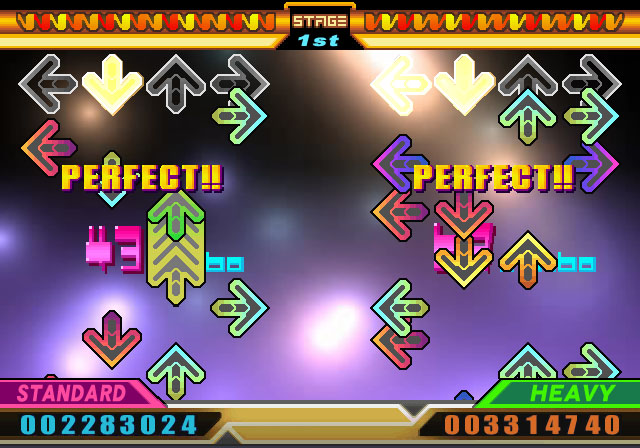
\includegraphics[width=0.43\textwidth]{Figures/dancedancerevolution}
  \end{center}
  \caption{Screenshot from \textit{Dance Dance Revolution}, an example of a rhythm music game~\cite{DDR}.}
  \label{fig:DDR}
\end{wrapfigure}

A music video game can be defined as a type of game that uses music or rhythm as an integral part of gameplay. This may involve pressing buttons in time with a song, whether on a conventional controller, and instrument controller or some kind of dance mat, singing into a microphone or creating original music. Players can often perform different parts of the same song together in local multiplayer games or over the Internet, providing enjoyable social experiences~\cite{mvgdef}.

Some games exhibit a sandbox style that encourages a free-form gameplay approach whereas other a hybrid style, which combines musical elements with more traditional genres, for example puzzle games or shooters. 

Below we will briefly go over different types of music video games that can be found on the market.


\vspace{10pt}


\subsection{Music Memory Games}

The goal of the music memory game is to score a player on their musical memory. Music track is presented to the user who then has to provide an appropriate response to each prompt from the game. Games may be based on different primary musical aspect (whether it is the rhythm, pitch or volume). However, a vast majority of the releases available on the market are rhythm-based.

\begin{figure}
        \centering
        \begin{subfigure}[b]{0.48\textwidth}
                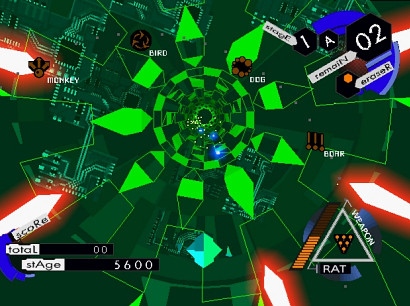
\includegraphics[width=\textwidth]{Figures/is}
                \caption{\textit{is -- Internal Section} -- an example of a generative hybrid music game~\cite{is}.}
                \label{fig:is }
        \end{subfigure}%
        ~ %add desired spacing between images, e. g. ~, \quad, \qquad, \hfill etc.
          %(or a blank line to force the subfigure onto a new line)
        \begin{subfigure}[b]{0.48\textwidth}
                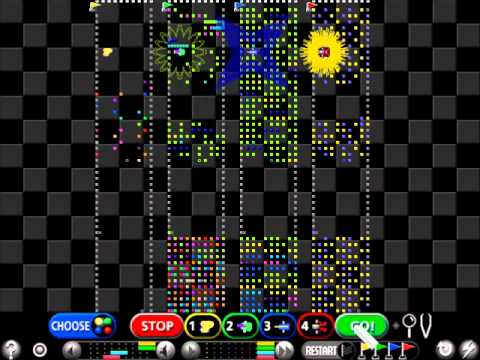
\includegraphics[width=\textwidth]{Figures/simtunes}
                \caption{\textit{SimTunes} -- an example of a free form music game~\cite{simtunes}.}
                \label{fig:simtunes}
        \end{subfigure}
          \caption{Examples of music video games.}
        ~ %add desired spacing between images, e. g. ~, \quad, \qquad, \hfill etc.
        \label{fig:simtunesandis}
\end{figure}


Rhythm games typically focus on dance or the simulated performance of musical instruments, and require players to press buttons in a sequence dictated on the screen. Doing so causes the game's protagonist or avatar to dance or to play their instrument correctly, which increases the player's score~\cite{rhythmgame}. An example of such games could be \textit{Guitar Hero} or \textit{Dance Dance Revolution}.

\vspace{10pt}


\subsection{Hybrid Music Games}

Hybrid music games are characterised by substantial and meaningful interactions between a player and the music game in a game that apparently belongs to a non-musical genre. This type of games can be further split into two sub-types.


Generative music video games make use of user’s actions. By monitoring interaction with the surroundings in the game, the mechanism generates sounds that are then integrated into the soundtrack, permitting the player’s direct interaction with the score. This encourages the creation of a synesthetic experience -- when upon stimulation of one sense others activate, causing an involuntary experience. An example of such game could be \textit{Rez}, which is a simple rail shooter. However, thanks to integrating sounds generated by player completing the normal task of rail-shooting, the musical score is dynamic.

Reactive music games, in contrast to generative one, employ music to determine the gameplay. In such games, the player takes cues from soundtrack to devise his gameplay. For example, \textit{iS -- Internal Section}, uses the music to determine the dynamics of the non-musical components of the game.

\vspace{10pt}


\subsection{Free Form Music Games}

In free form music games, the main task of the user is to create content. This form of music game is often compared to non-game music synthesisers. Free form music games are somewhere between generative hybrid music games and non-game utilities, depending on the degree to which their gameplay relies on a driving underlying plot-line. An example of such game could be \textit{SimTunes}, where the user is painting a picture using large pixels and each colour represents a musical note. 

\begin{figure}
        \centering
        \begin{subfigure}[b]{0.48\textwidth}
                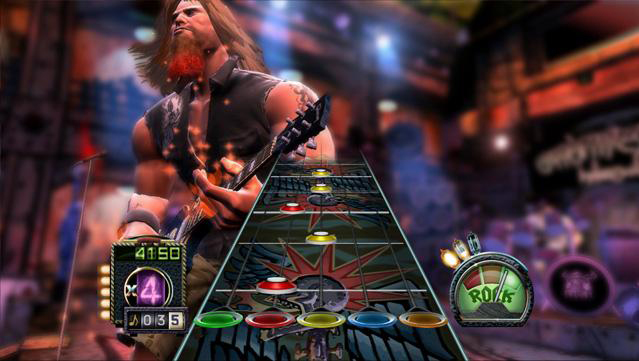
\includegraphics[width=\textwidth]{Figures/guitarhero}
                \caption{Screenshot from \textit{Guitar Hero} -- player is attempting to play a song~\cite{ghscreen}.}
                \label{fig:Guitar Hero screenshot}
        \end{subfigure}%
        ~ %add desired spacing between images, e. g. ~, \quad, \qquad, \hfill etc.
          %(or a blank line to force the subfigure onto a new line)
        \begin{subfigure}[b]{0.48\textwidth}
                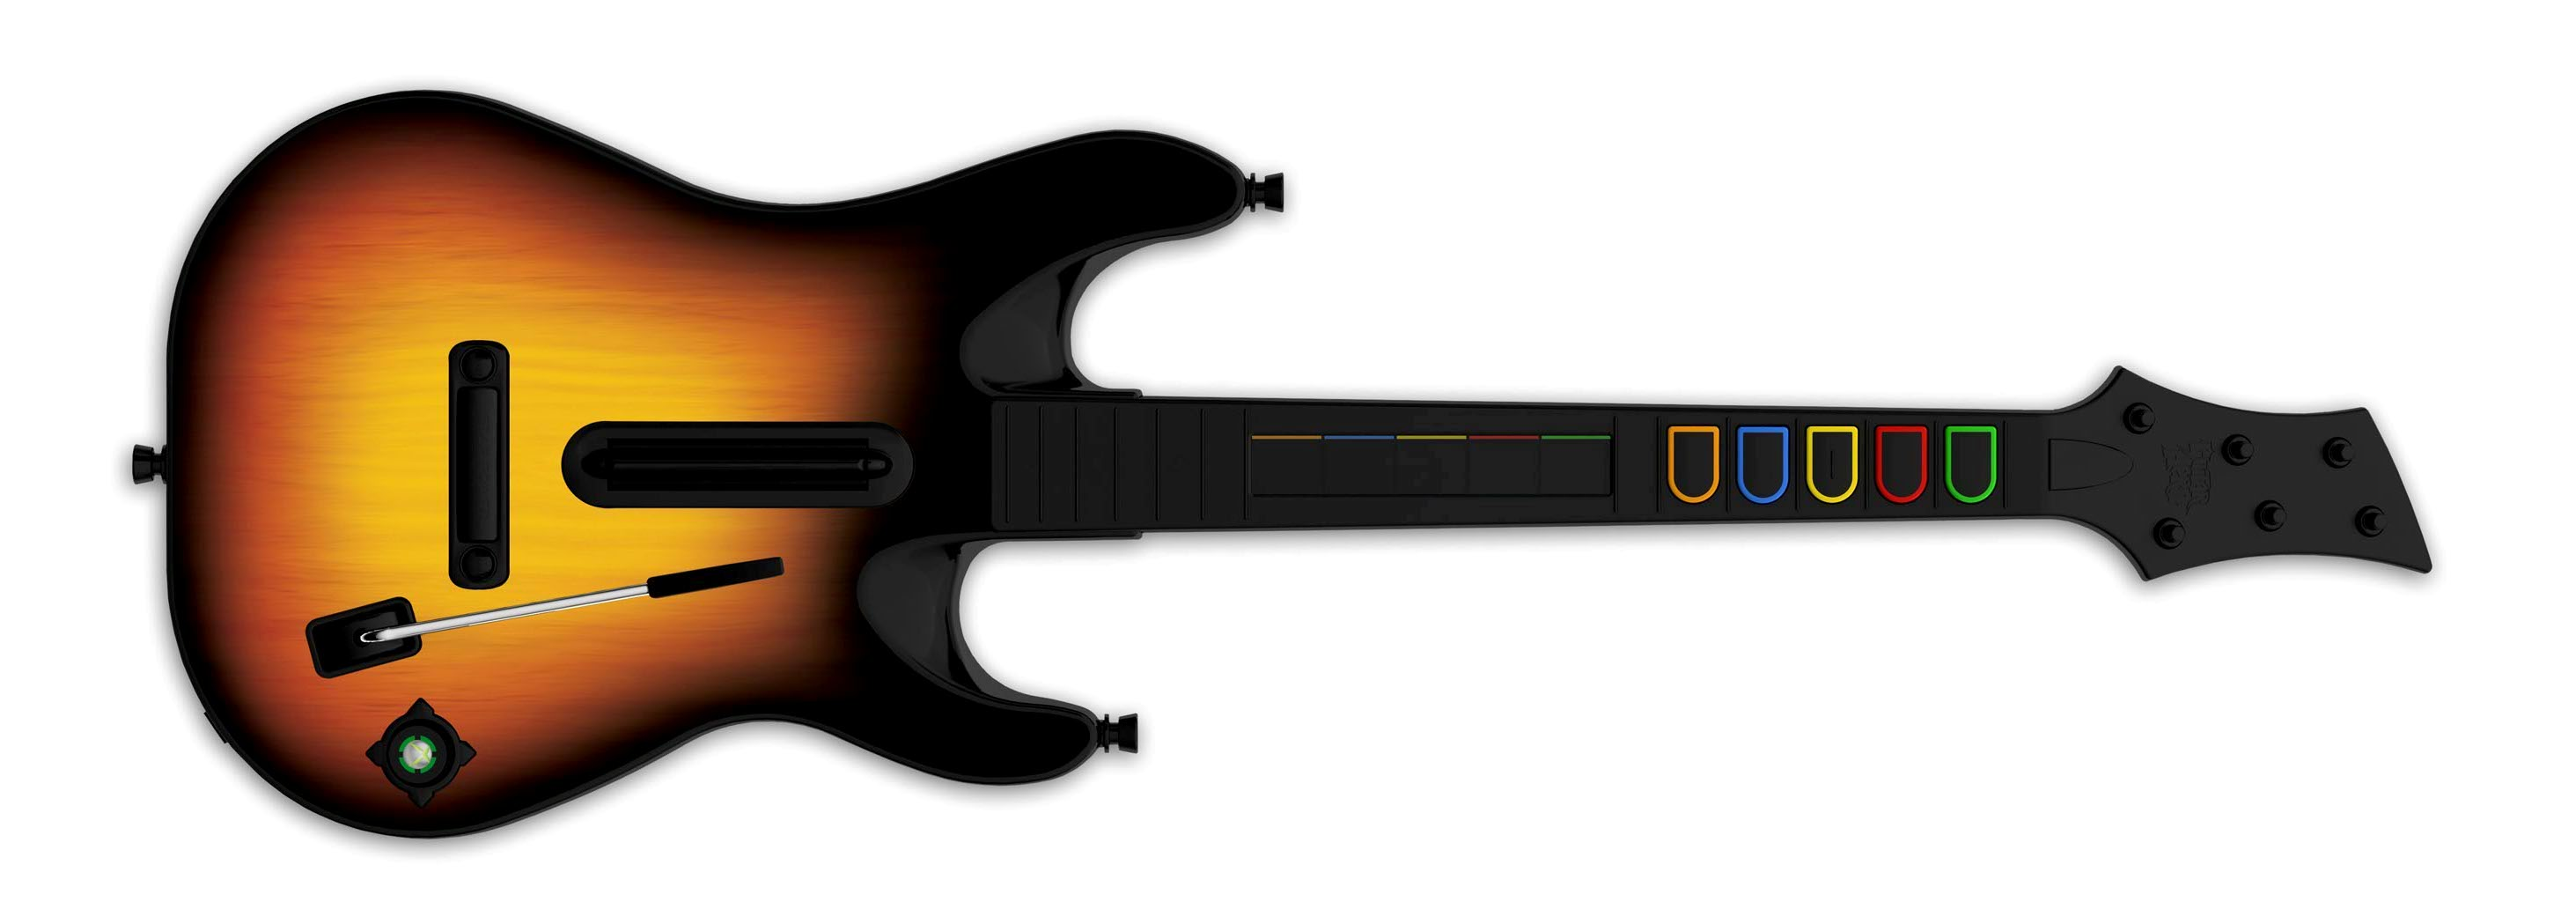
\includegraphics[width=\textwidth]{Figures/controller}
                \caption{A guitar shaped controller used in the game~\cite{controller}.}
                \label{fig:Controller}
        \end{subfigure}
          \caption{Guitar Hero components}
        ~ %add desired spacing between images, e. g. ~, \quad, \qquad, \hfill etc.
        \label{fig:GH}
\end{figure}

\vspace{20pt}


\section{Case Study -- Guitar Hero}

Guitar Hero is one of the most popular franchises in the history of music games. The first of the series was published in 2005 by RedOctane and Harmonix. In the games, players use instrument-shaped game controllers to simulate playing the instruments across numerous rock music songs. It is widely considered a highly entertaining game fully embracing the concept of a rhythm-based music game.

\vspace{10pt}


\subsection*{The Controller}


Rather than a typical gamepad, Guitar Hero uses an instrument-shaped controller (guitar in the earlier releases, supplemented by bass, microphone and drums in more recent ones). Playing the game with the guitar controller simulates playing an actual guitar, except it uses five coloured ``fret buttons'' and a ``strum bar'' instead of frets and strings, and an analogous mapping for the other instruments. They incorporate most of the real life techniques and motions that an instrumentalist would perform on a real instrument.

\vspace{10pt}


\subsection*{The Gameplay}

The actual game itself works exactly as many other music titles do. At the bottom of the screen, a number of (varying depending of level of difficulty) buttons is shown. In each attempt, a series of notes moves across the screen and when a note aligns with a button, player is supposed to press a corresponding button, gaining points depending on the accuracy. If the player failed to achieve a certain amount of notes -- his performance meter stays low for a longer time, he loses the game.

However, there are a couple minor improvements that Harmonix has made to the general music game formula. By pressing buttons with really good accuracy in a song, a player is able to build up Star Power, which when unleashed, doubles up current point multiplier. Star Power also adds a bit of a strategic element -- player not only earns more points when it is activated, but he can also raise your performance meter faster, enabling him to last longer when encountering a trickier part of a song.

\vspace{10pt}


\subsection*{The Critique}

Without a doubt, Guitar Hero features a great selection of music. However, there will always be tracks missing, regardless of how many versions of Guitar Hero are released. People have different tastes and successfully limiting a game to a set of tracks that everybody is supposed to enjoy is a really hard task. 

Some more advanced users familiar with Computer Science attempted to transcribe songs and to create new levels. However, this process is really difficult, consisting of many laborious stages and requiring an additional midi files with separated guitar track. This discouraged an average user from fully making use of game’s capabilities. The producers, seeing the tendency, started releasing the in-app purchases to enable the players to extend their library and thus, keep the users. 

As there is a clear need for custom music extension to the game, implementing a feature of uploading some music preferred by the player would definitely improve user satisfaction. However, this has not been achieved yet as the task itself is quite complex. Moreover, enabling the users to load in some music would deprive the company of their income sources.

\vspace{30pt}
\newpage

\section{Introduction to Music Analysis}
\vspace{10pt}


Automatic music analysis is thought of as an automated extraction of relevant perceptual information (notes, instruments, etc.) from music files (like MP3 or WAV files). First attempted in the 1970s at Stanford University~\cite{moorer}, it remains an unsolved problem. The task is highly multifaceted and interdisciplinary, requiring the extraction of musical notes, instruments, percussion, emotion, etc., and drawing from fields as varied as computer science, mathematics, biology, physics, psychology, and electrical engineering. The problem's difficulty lies in a necessity to reverse-engineer the human brain. 

In this section we go over the basic terminology used in music analysis.

\vspace{10pt}

\subsection{Sound Spectrum}

\begin{wrapfigure}{r}{0.5\textwidth}
  \vspace{-50pt}

  \begin{center}
    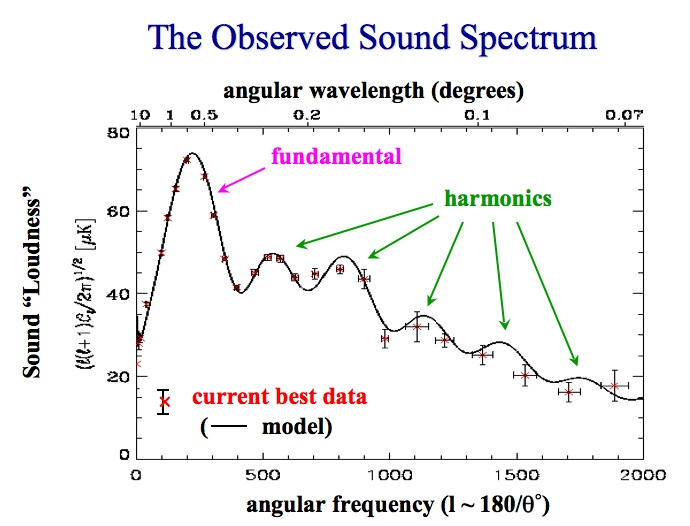
\includegraphics[width=0.48\textwidth]{Figures/soundspectrum}
  \end{center}
  \caption{Example of a sound spectrum diagram~\cite{soundspectrum}.}
  \label{fig:soundspectrumexample}
\end{wrapfigure}


Most sounds are made up of a complicated mixture of vibrations. A sound spectrum is a representation of a sound – usually a short sample of a sound – in terms of the amount of vibration at each individual frequency. It is usually presented as a graph of either power or pressure as a function of frequency. The power or pressure is usually measured in decibels and the frequency is measured in vibrations per second (or hertz, abbreviation Hz) or thousands of vibrations per second (kilohertz, abbreviation kHz). 

\vspace{10pt}

\subsection{Pitch, Tones, Fundamental Frequency, Timbre}

Pitch is the most natural way of ordering sounds on a frequency-related scale. If sounds have a frequency which is clear and stable enough to be distinguished from noise, they can be compared between one another as “lower” or “higher”. Pitch is not an objective physical property — it depends on anatomy and physiology of the auditory system, which is a subject of an extensive study called psychoacoustics~\cite{pitch}. 

A semitone is the smallest musical interval commonly used in Western tonal music. Two semitones constitute a tone.

The fundamental frequency $f_{\text{0}}$ is defined as the lowest frequency of a periodic waveform. A harmonic (or a harmonic partial) is any of a set of partials that are whole number multiples of a common fundamental frequency. This set includes $f_{0}$, which is a whole number multiple of itself (1 times itself).

Fundamental frequency can be thought of as the physical property most closely related to perception of pitch. This is why in this context pitch and fundamental frequency can be used interchangeably~\cite{salamon}.

Timbre is what makes a particular musical sound different from another, even when they have the same pitch and loudness. For instance, it is the difference between a guitar and a piano playing the same note at the same loudness. Experienced musicians are able to distinguish between different instruments of the same type based on their varied timbres, even if those instruments are playing notes at the same pitch and loudness.

\vspace{10pt}

\subsection{Polyphonic Music}

Polyphony is a word derived from Greek \textit{poluph\={o}nosis} meaning more than one sound — a texture consisting of two or more simultaneous lines of independent melody~\cite{polyphonic}. This is usually contrasted with homophony, where musical parts move in the same rhythm and one dominant melodic voice is accompanied by chords or monophony, where only one voice is found. 

However, in our case, the term polyphonic will simply refer to any type of music in which two or more notes can be played simultaneously. This effect be achieved either by playing in different instruments (for example, voice, guitar and bass) or a single instrument capable of playing more than one more at a time (like a piano).

\vspace{10pt}

\subsection{Melody}

The concept of “melody” ultimately relies on the judgement of people listening. This is why it varies depending on the application context -- whether we want to determine symbolic melodic similarity or transcribe a music track. 

In order to have a clear framework to work within, the Music Information Retrieval (MIR) community has adopted in recent years the definition proposed by~\cite{melodydef}, ``...the melody is the single (monophonic) pitch sequence that a listener might reproduce if asked to whistle or hum a piece of polyphonic music, and that a listener would recognise as being the 'essence' of that music when heard in comparison''.

In practice, research has focused on ``single source predominant fundamental frequency estimation'' — which means a search for a main melody coming from a single sound source throughout the song analysed. As we can see, the subjective element is still present in this description of a melody as there might not be a definite way of deciding what predominant is. However, it fits well with our project’s objective — generating a game level based on changes in the pitch.

\vspace{10pt}

\subsection{Filter}

Any medium through which the music signal passes, whatever its form, can be regarded as a filter. However, we do not usually think of something as a filter unless it can modify the sound in some way. 

A digital filter is a filter that operates on digital signals, such as sound represented inside a computer. It is a computation which takes one sequence of numbers (the input signal) and produces a new sequence of numbers (the filtered output signal)~\cite{filters}.

\vspace{10pt}

\subsection{Short Time Fourier Transform}

Short-time Fourier transform (STFT), is a signal processing method which is used in analysis of non-stationary signals with statistic characteristics varying with time.
In particular, STFT extracts several frames of the signal to be analysed with a window that moves with time. If we set the window size to be narrow enough, each frame extracted can be viewed as stationary so that Fourier transform can be used. With the window moving along the time axis, the relation between the variance of frequency and time can be identified~\cite{STFT}.
Mathematically, this is written as:
\begin{equation}
\mathbf{STFT}\{x(t)\}(\tau,\omega) \equiv X(\tau, \omega) = \int_{-\infty}^{\infty} x(t) w(t-\tau) e^{-j \omega t} \, dt 
\end{equation}
where $w(t)$ is the window function, commonly a Hann window or Gaussian window bell centered around zero, and $x(t)$ is the signal to be transformed. 

The short time Fourier transform of a time-domain signal $y$ is denoted by the matrix $F \times N$, $F$ being the Fourier transform size and $N$ the number of analysis frames.

\vspace{10pt}

\subsection{Chroma}

\begin{figure}       
      \centering
                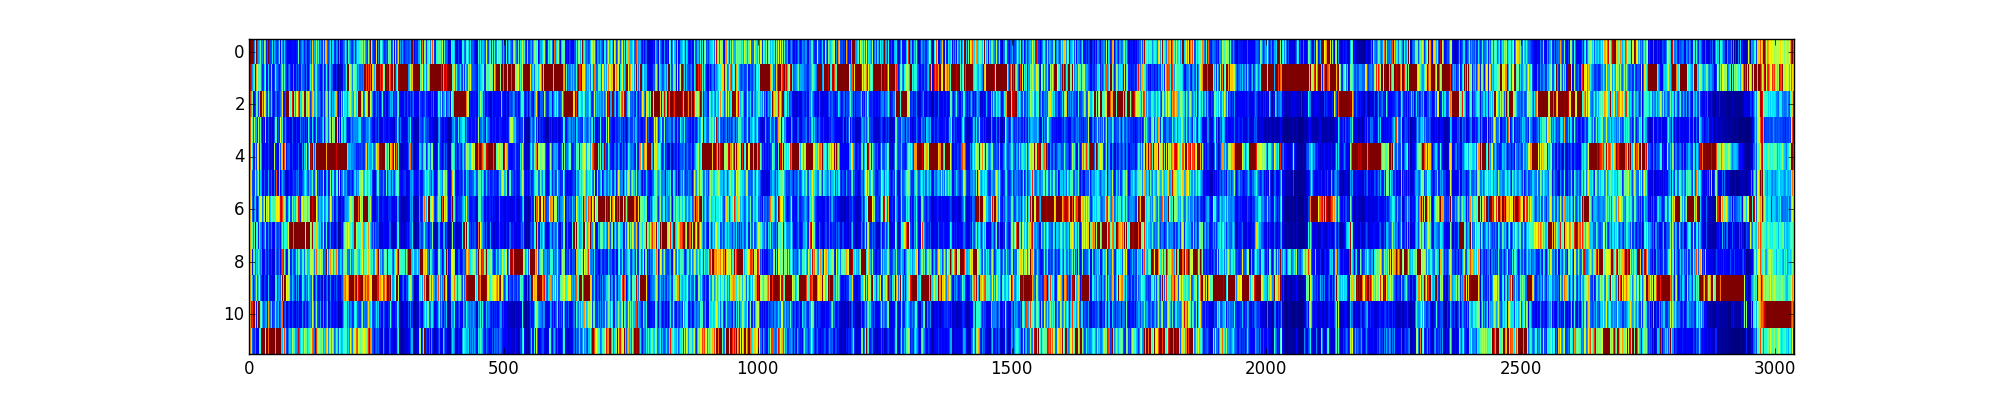
\includegraphics[width=\textwidth]{Figures/chromagram_example}
			   \vspace{15pt}
			   \label{fig:chromaexample}
			   \caption{Example of a chromagram, generated for ``Help!'' by The Beatles. The blue spots represent small amount of energy and the dark red stand for the high energy in each pitch at given time.}
\end{figure}

A chroma feature is characterised by a 12-dimensional vector representing the amount of energy that can be found in each of different pitches at said time. We usually consider the 12 pitches commonly existing in the western popular music folded into one single octave, but one can use multiples of 12 to take the semi-tones or even smaller differences between tones into account. We achieve that by applying a Constant Q Transform across the entire spectrogram. 

In mathematics and signal processing, the Constant Q Transform transforms a data series to the frequency domain. It is related to the Fourier Transform, and very closely related to the complex Morlet wavelet transform~\cite{wavelet}. 

The transform can be thought of as a series of logarithmically spaced filters, with the $k$th filter having a spectral width some multiple of the previous filter's width, i.e.

\begin{equation}
\delta f_k = 2^{ \frac {1}{n} } * \delta f_{k-1} = \left ( {2^{ \frac {1}{n} }} \right )^{k} * \delta f_{\mathrm{min}}
\end{equation}

where $\delta f_{k}$ is the bandwidth of the $k$th filter, $f_{min}$ is the centre frequency of the lowest filter, and $n$ is the number of filters per octave.

Next, the spectrogram is folded into one octave comprising the $M$ quantised pitches, where $M$ is the number of pitches found in the chroma. When these features are stack together following the song structure in a $N \times M$; matrix, a chromagram is generated, where N is the number of time frames in which the musical piece has been divided~\cite{constantQ}.

\vspace{20pt}
\newpage

\section{Main Melody Extraction from Polyphonic Music}
\vspace{10pt}
\label{sec:mainmelodybackground}

For a long time people were researching ways of estimating the fundamental frequency, be it with monophonic music recording or multi-pitch estimation. Melody extraction differs from both of those problems. Unlike monophonic pitch estimation, it handles polyphonic tracks. In contrast to multi-pitch estimation, it must also include a mechanism for source identification, to spot the voice carrying the melody within the polyphony, as the main focus of these algorithms is to estimate the main melody from a single source. 

To be able to evaluate the performance of the new algorithms, annual Music Information Retrieval Evaluation eXchange (MIREX) has been running since 2005. In this campaign, different models are evaluated against the same sets of music collections in order to obtain a quantitative comparison between methods and assess the accuracy of the current state-of-the-art in melody extraction~\cite{comparison}.

In this section we will go over two different approaches to the problem of main melody extraction from polyphonic music, using source separation and a salience function. Then we will compare both methods to help determine which one is more suitable for our project.

\vspace{10pt}

\subsection{Source Separation Based Approach}

\begin{wrapfigure}{r}{0.6\textwidth}
\vspace{-30pt}
  \begin{center}
    \includegraphics[width=0.58\textwidth]{Figures/durrieudiagram}
  \end{center}
  \caption{Outline of system proposed by Durrieu: X is the STFT of the mixture signal, $p(\Xi|X)$ the posterior probability of a given melody sequence, and $\hat{\Xi} $ the desired smooth melody sequence~\cite{durrieu}.}
  \label{fig:durrieu}
\end{wrapfigure}

In polyphonic tracks the main melody can be represented by a specific source/filter model. In case of the leading vocal part, the vocal cords are treated as a source and the voice tract as a linear acoustic filter.

In their paper from 2011~\cite{durrieu}, Durrieu together with Richard, David and Fevotte, presented an algorithm in which they assume that at any given time the music signal observed is a mixture of two elementary signals -- one corresponding to the main source and one to the background music. Therefore, the signal can be represented in an equation $x(t) = v(t) + m(t)$, where $v(t)$ stands for the source of the main melody and $m(t)$ is the background music. Interestingly, this equation also holds for the short-time Fourier transform (STFT)  $X$, $V$ and $M$ respectively: $X = V + M$. The models proposed by Durrieu aim at constraining the shapes of these STFT using temporal and spectral constraints. 

The likelihood of the vocal part $V$ is calculated using two different frameworks. 

The first one uses the source/filter Gaussian scaled mixture model (GSMM). 

In short, a Gaussian mixture model is a probabilistic model that assumes all the data points are generated from a mixture of a finite number of Gaussian distributions with unknown parameters. We can think of mixture models as generalizing k-means clustering to incorporate information about the covariance structure of the data as well as the centers of the latent Gaussians. For description of k-means clustering, we refer to Section~\ref{sec:kmeans}.

In this GSMM model, the source element refers to the excitation of the vocal folds. This is why it is linked to the fundamental frequency of the sound $f_{\text{0}}$. On the other hand, the filter part is characteristic of the vocal tract shape. This space of possibilities is then discretised so that one possible filter frequency response is considered. It is then used to calculate the likelihood of the vocal part knowing the filter and $f_{\text{0}}$.

\begin{figure}[b]
        \centering
        \begin{subfigure}[b]{0.48\textwidth}
                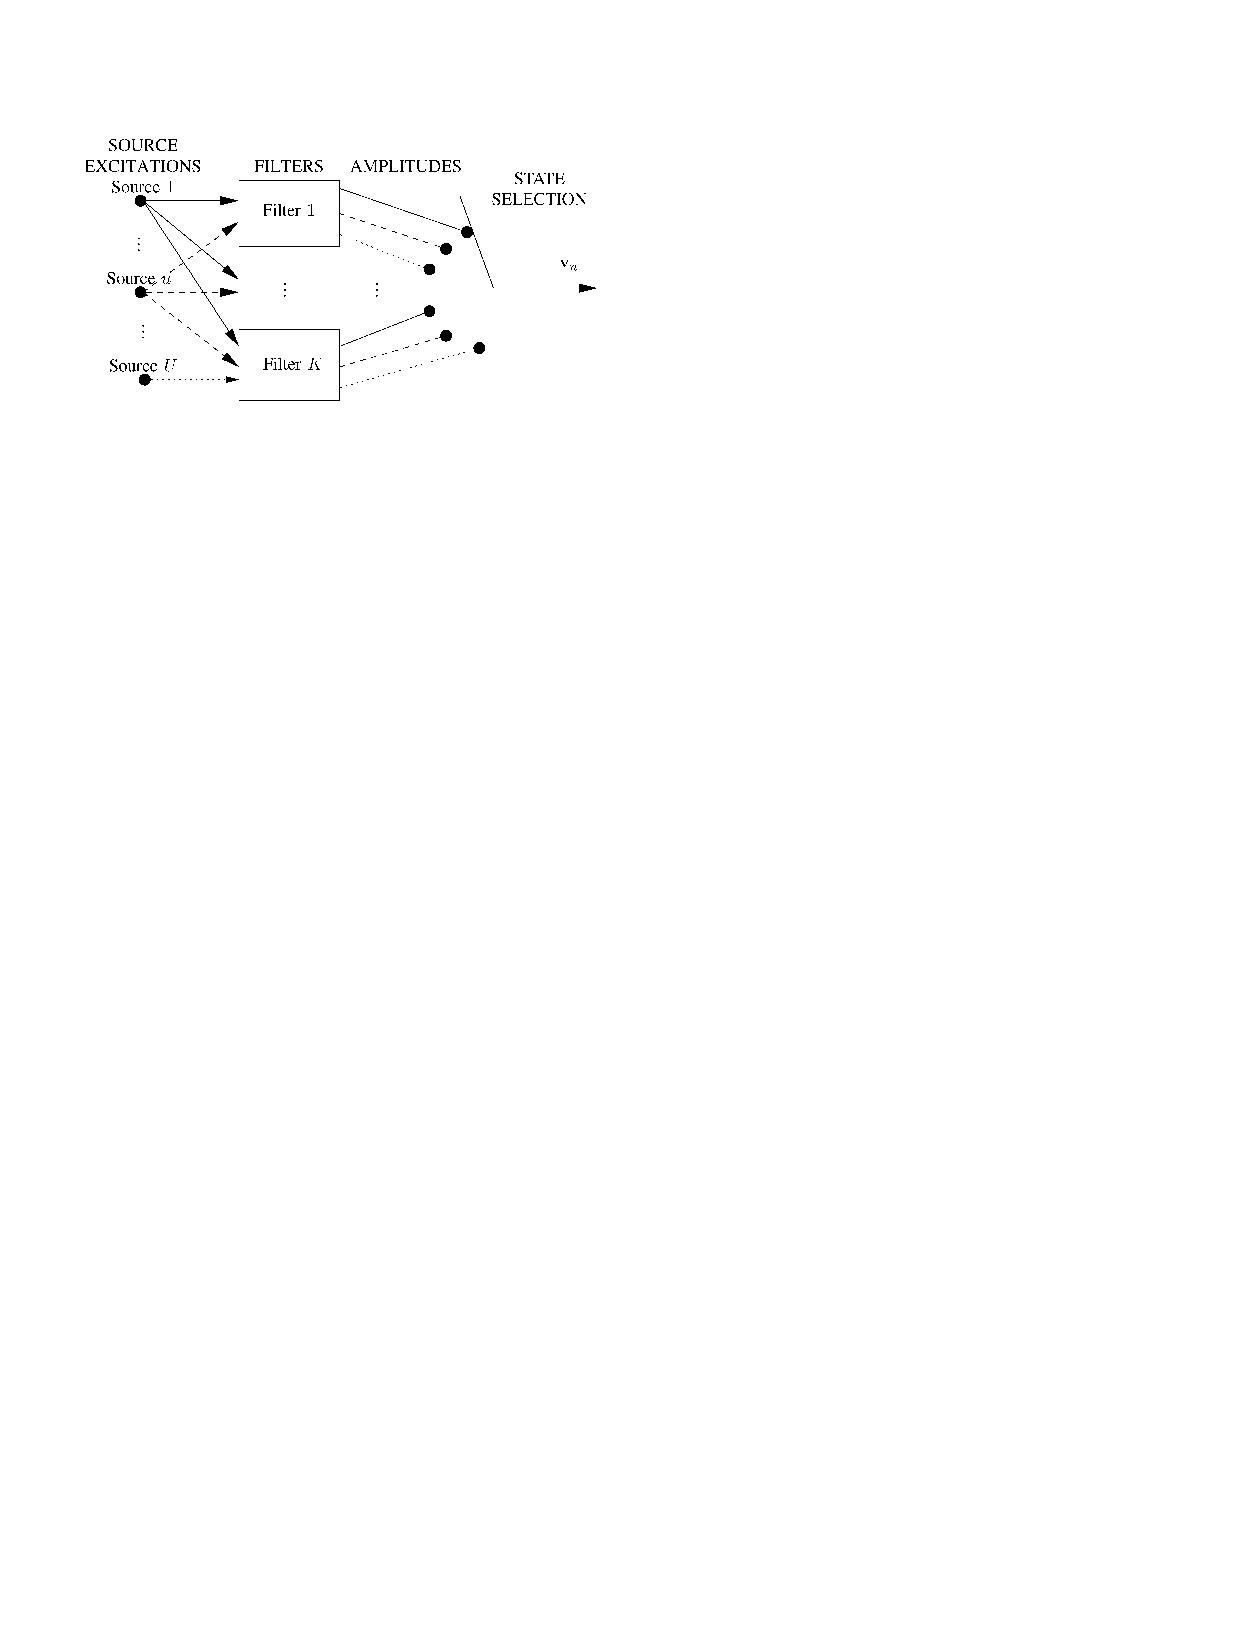
\includegraphics[width=\textwidth]{Figures/gsmm}
                \caption{Schematic principle of the generative GSMM. Each source u is filtered by each filter $k$. For frame $n$, the signal is then multiplied by a  given amplitude and a ``state selector'' then chooses the active state.}
                \label{fig:gsmm}
        \end{subfigure}%
        \begin{subfigure}[b]{0.48\textwidth}
                \includegraphics[width=\textwidth]{Figures/imm}
                \caption{Schematic principle of the generative IMM. At each frame, all the $U$ sources, each filtered by $K$ filters, are multiplied by amplitudes and added together to produce the leading voice signal.}
                \label{fig:imm}
        \end{subfigure}
          \caption{Diagram of both models presented in the paper~\cite{durrieu}.}
        \label{fig:gsmmimm}
\end{figure}

Figure~\ref{fig:gsmm}  A) shows the diagram of the GSMM model for the main voice part. Each source excitation $u$ is filtered by each filter $k$. The amplitudes for a frame $n$ and for all the couples $(k, u)$ are then applied to each of the output signals. At last a ``state selector'' sets the active state for the given frame.

The second model was derived from the first one to find a solution that would be more efficient to compute. The authors came up with a formulation that keeps the source/filter model within an instantaneous mixture framework (IMM). In this model, for each source a set of filters is defined and at each frame, once every source is filtered and multiplied by a given amplitude, they are all added together.

Then the likelihood of the background music is calculated.

The background music signal $m(t)$ can be thought of as a mixture of $R$ independent Gaussian sources $m_{r}(t)$. Each of the sources is centred and characterised by its power spectral density (PSD), which describes how the power of a signal or time series is distributed over the different frequencies. PSD can be estimated using a Covariance Method.

Due to the linearity of the Fourier transform, $M(f,t)$, the STFT of $m$, is also the instantaneous mixture of the $R$ spectra $M(f,t)$ of the sources: $M_{r}(f,t)$.
This together with STFT and an amplitude coefficient associated with each source is used to calculate the likelihood for each of the frequency bins. Let $M_{t}(f)$ be the STFT of the background signal at frame $t$ and frequency bin $f$, then we calculate its likelihood.

Once the parameters are estimated using the maximum likelihood criterion for each of the model, the Viterbi smoothing of the melody line is applied, obtaining a trade-off between the smoothness of the melody and its global energy in the signal. The Viterbi algorithm is a dynamic programming algorithm for finding the most likely sequence of hidden states – called the Viterbi path – that results in a sequence of observed events~\cite{viterbi}.
 
The authors then parametrise the transitions between the possible main melody without disabling jumps from one note to the other. Using Wiener filtering a framework is implemented to separate the source. Wiener filtering is a digital signal processing method which reduces noise level by applying a statistical estimate of the signal using a desired data without such noise. This way separated signals are obtained. Computing the energy for each frame of the separated main melody and thereafter thresholding allowed the authors to discriminate between spurious notes and true positives.

\vspace{20pt}


\subsection{Salience Based Approaches}

\begin{wrapfigure}{r}{0.6\textwidth}
  \vspace{-30pt}
  \begin{center}
    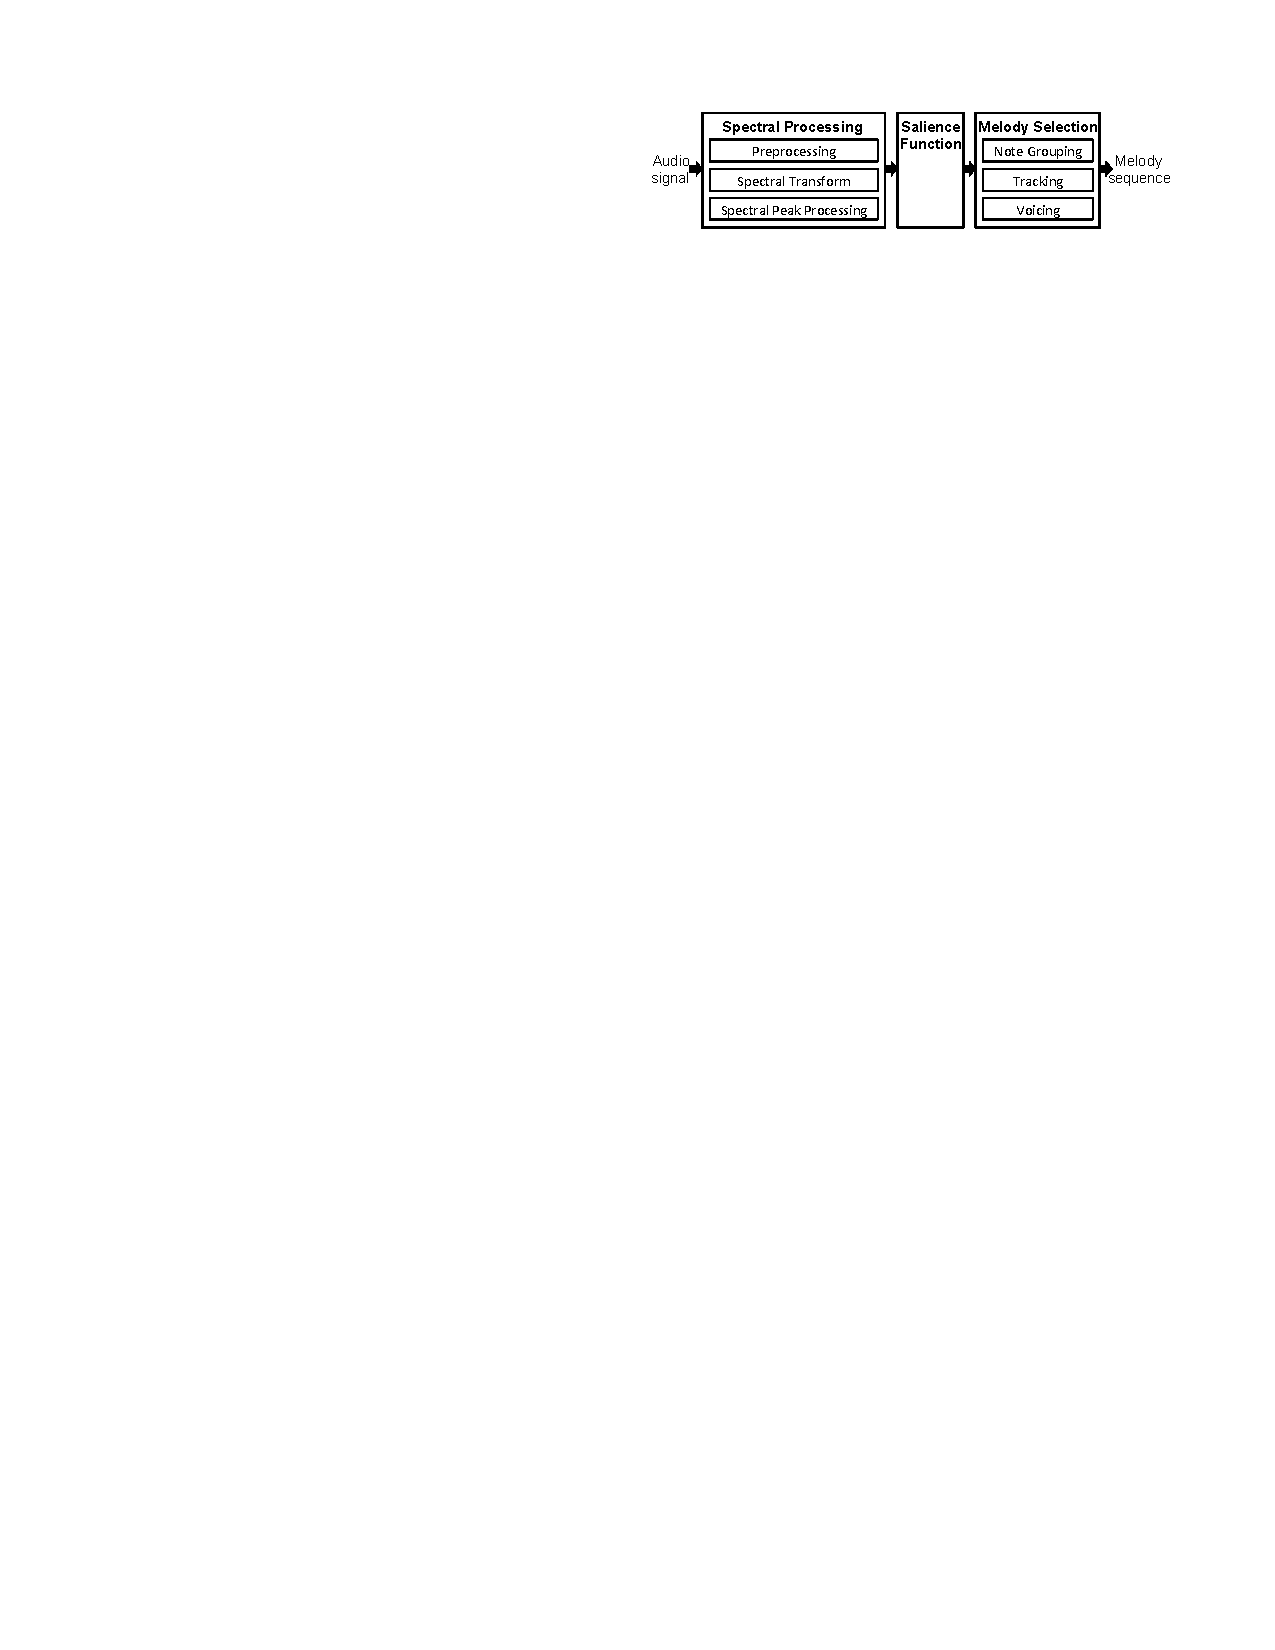
\includegraphics[width=0.58\textwidth]{Figures/salienceoveralldiagram}
  \end{center}
  \caption{Block diagram of four main blocks of the system by Salamon and G\'{o}mez: sinusoid extraction, salience function computation, pitch contour creation and melody selection~\cite{comparison}.}
  \label{fig:3stepsalience}
\end{wrapfigure}

This type of approach has been the most popular so far, with majority of algorithms evaluated at MIREX implementing it. It can be split into several smaller stages, as seen in Figure~\ref{fig:3stepsalience}. In particular, a method implemented in paper~\cite{salamon} seems to be quite promising.

Usually in salience based approaches, as a first step some sort of pre-processing is applied to the audio signal to enhance the frequency content where one expects to find the melody. In particular, Salamon and G\'{o}mez apply an equal loudness filter, which enhances the frequencies to which the human ear is more perceptually sensitive, by taking a representative average of the equal loudness curves and filtering the signal by its inverse. 

This stage is followed by a spectral transform — the signal is chopped into time frames and a transform function is applied to obtain a spectral representation of each frame.
This is achieved by applying the short-time Fourier transform given by:

\begin{equation}
X_{l}(k) = \sum_{n=0}^{M-1} w(n) \times x(n + lH) e^{-j\frac{2 \pi}{N}kn}
\end{equation}

with a window length of 46.4ms. Here, $x(n)$ is the time signal, $w(n)$ the windowing function, $l$ the frame number, $M$ the window length, $N$ the FFT length and $H$ the hop size. Thanks to choosing a relatively small hop size, Salamon and G\'{o}mez achieve sufficient frequency resolution to identify different notes while maintaining adequate time resolution to track pitch changes in the melody over a short time. 

Having done this, the authors move to frequency/amplitude correction, where the spectral peaks are detected and used to construct a salience function. To avoid a relatively large error in the estimation of the peak frequency caused by binning them in the process of FFT, peak’s instantaneous frequency and amplitude are calculated. 

As we can see in Figure~\ref{fig:3stepsalience}, those three steps constitute the spectral processing. But at the core of the salience based algorithms lies the multi-pitch representation, i.e. the salience function. A salience function provides an estimation of the predominance of different fundamental frequencies (or pitch classes) in the audio signal at every time frame. The peaks of this function form the $f_{0}$ candidates for the main melody. In the algorithm described by Salamon and G\'{o}mez, this computation is based on harmonic summation, where the salience of  a given frequency is computed as a sum of the weighted energies found at harmonics (integer multiples) of that frequency. Using only the peaks for the summation allows the authors to discard less reliable values and apply further frequency corrections. 

\begin{figure}[t]
  \centering
    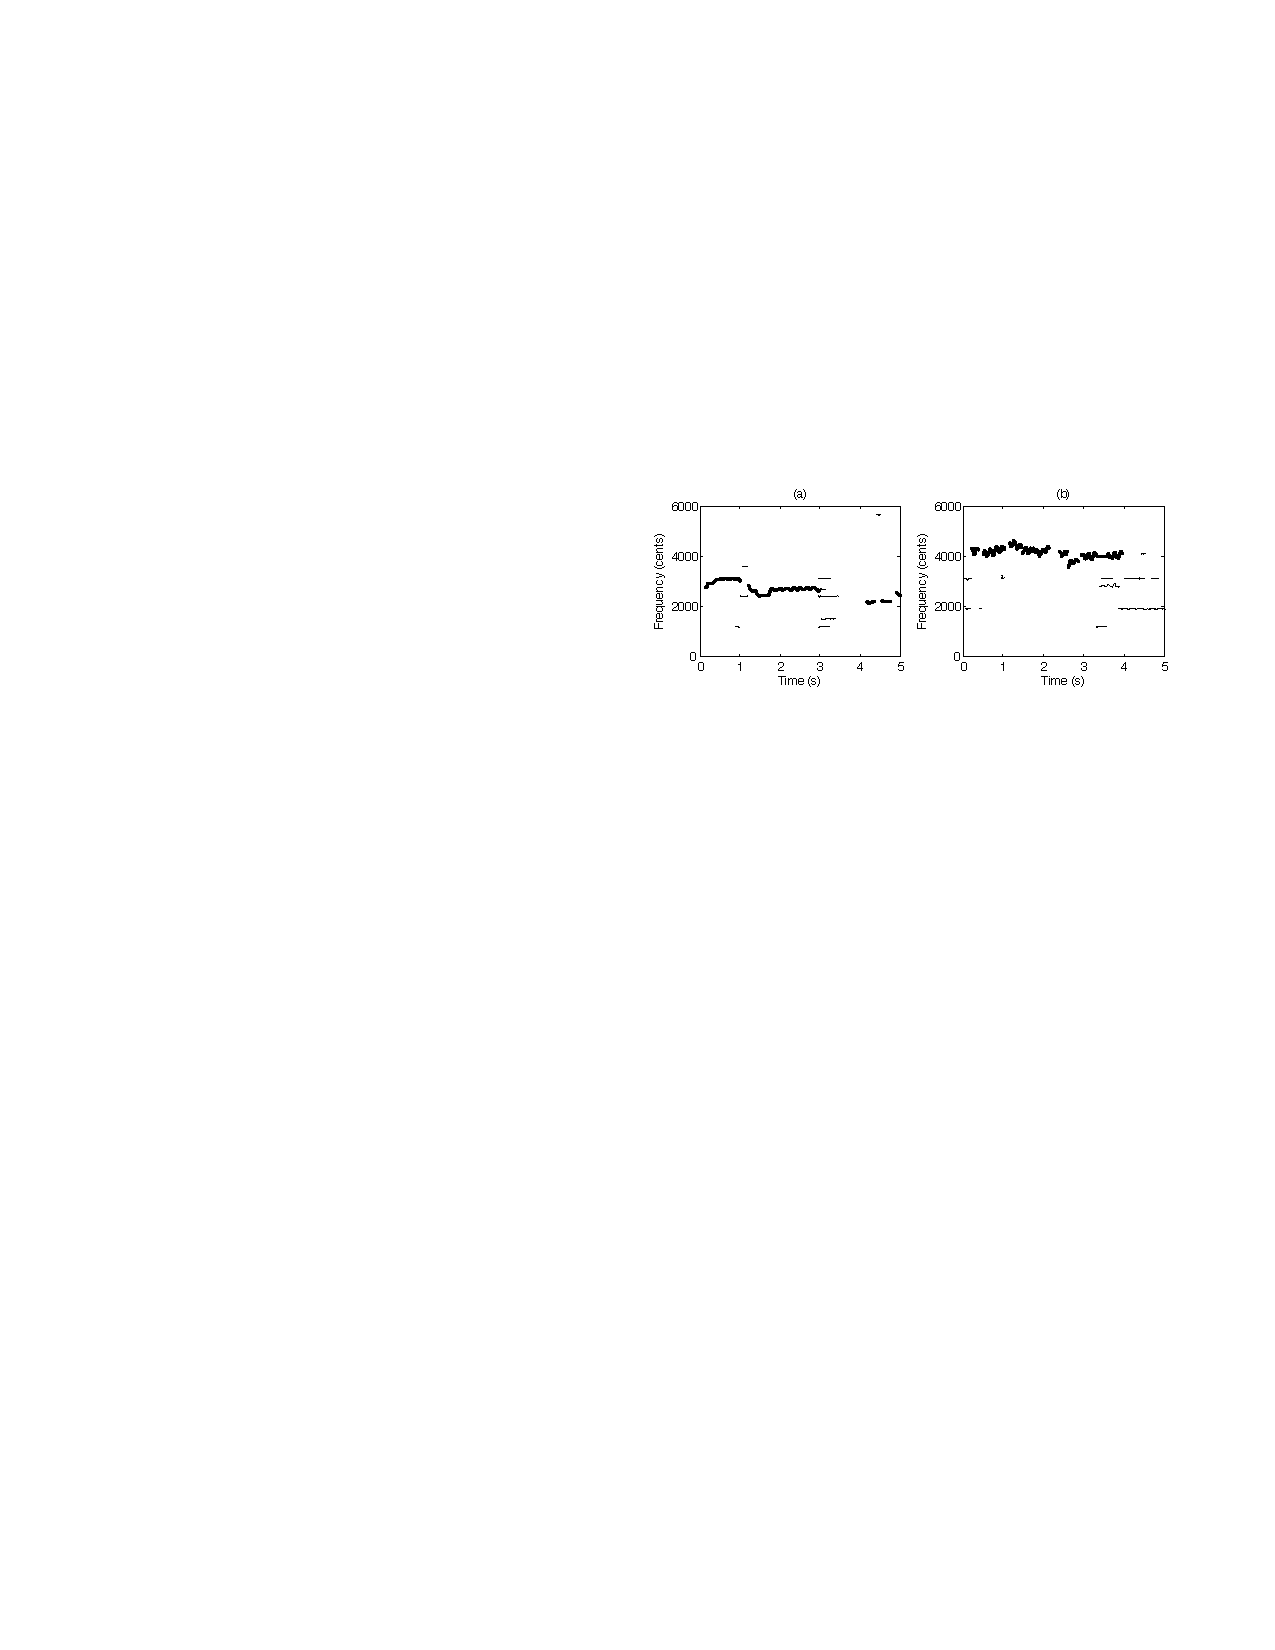
\includegraphics[width=0.8\textwidth]{Figures/pitchcontour}
      \caption{Pitch contours generated from excerpts of (a) vocal jazz and (b) opera. Melody contours are highlighted in bold~\cite{salamon}.}
\label{fig:pitchcontours}
\end{figure}

The salience function presented in the paper covers a pitch range of nearly five octaves from 55Hz to 1.76kHz.

After this step, the peaks of the salience function at each frame are potential $f_{0}$s of the main melody. At this point, some methods for melody extraction attempt to track the melody. However, Salamon and G\'{o}mez filter out the non-salient peaks, first by comparing them to the highest peak in the frame and then to a value computed using salience mean and standard deviation of all remaining peaks (in all frames). Then the peaks are grouped into pitch contours -- time and pitch continuous sequences of salience peaks, as shown in Figure~\ref{fig:pitchcontours}.

\begin{figure}
  \begin{center}
    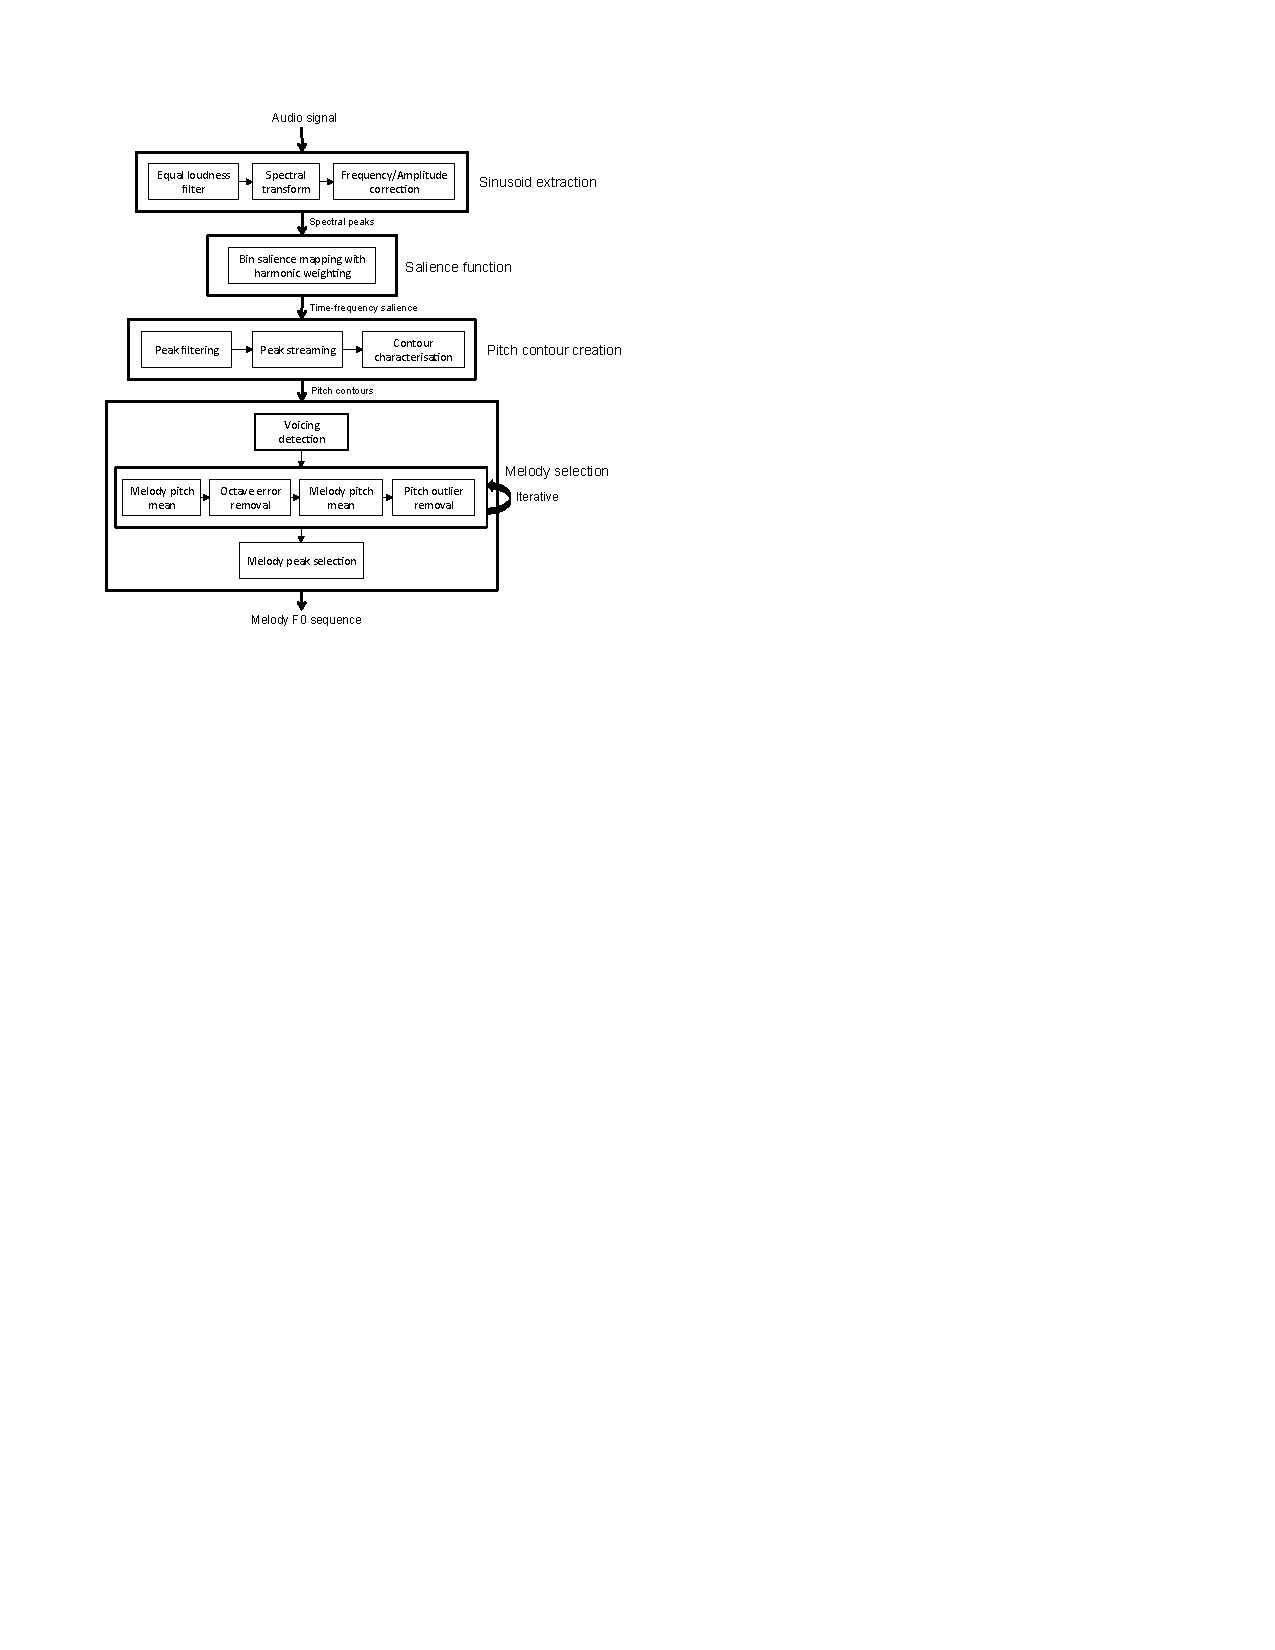
\includegraphics[width=0.75\textwidth]{Figures/salamon4blocksdiagram}
  \end{center}
  \caption{Block diagram of four main blocks of the system by Salamon and G\'{o}mez: sinusoid extraction, salience function computation, pitch contour creation and melody selection~\cite{salamon}.}
\end{figure}

Having created the pitch contours, Salamon and G\'{o}mez are faced with the task of determining which one belongs to the main melody. The authors define features based on contour pitch, length and salience, that will later guide the selection process. The process is initiated by grouping peaks into continuous pitch contours, out of which a melody is selected later. 

The next main block in this algorithm shown in Figure~\ref{fig:3stepsalience} is the melody selection which is comprised of three steps: voicing detection, octave error minimisation/pitch outlier removal, and final melody selection. The first one, the voicing detection, is tasked with determining when the main melody is present. 

To filter out some of the contours that are present when the main melody is absent, Salamon and G\'{o}mez take advantage of the contour mean salience distribution. By setting the threshold to a value slightly below the average contour mean salience of all contours in the excerpt $C_{s}$, they manage to filter out a considerable amount of non-melody contours. The authors define the following voicing threshold $\tau_{v}$ based on the distribution mean $C_{s}$ and its standard deviation $\sigma_{\overline{s}}$:
\begin{equation}
\tau_{v} = C_{s} - v \times \sigma_{\overline{s}}
\end{equation}

The parameter $v$ determines the lenience of the filtering -- a high $v$ value might keep the false melody contours and a low value might filter out the melody contours.

It is also important to note that detecting certain characteristics in the contour increases a probability of it being the melody contour, for example in case of detecting a vibrato -- a regular, pulsating change of pitch, used to add expression to vocal and instrumental music~\cite{vibrato}

Next step in the melody selection, described by Salamon and G\'{o}mez in their paper, is octave errors and pitch outliers removal. In particular, the octave errors are the main sources of errors in melody extraction systems, when a multiple or sub-multiple of $f_{0}$ is reported as the main melody. To detect such errors, contour trajectories are compared by computing distance between their values on a per-frame for the region they overlap in and computing the mean over this region. If the mean distance is within $1200\pm50$ cents, the contours are considered octave duplicates.

Secondly, Salamon and G\'{o}mez use the relationship between contours neighbouring in time to decide which of the duplicates is the correct one. Their approach is based on two assumptions: firstly, that most (though not all) of the time the correct contour will have greater salience than its duplicate (the salience function parameters were optimised to this end). Secondly, that melodies tend to have a continuous pitch trajectory avoiding large jumps, in accordance with voice leading principles.

The method iteratively computes the $\overline{P(t)}$ -- pitch trajectory that represents the time evolution of the melody's pitch. It then detects and removes an octave duplicate as well as  the ``pitch outliers'' -- contours more than one octave above or below the pitch mean and then it is recalculated. Authors empirically discovered that 2 iterations of this process are enough to get a good approximation of the true trajectory of the melody, which is then passed to the final stage of the model -- the final melody selection.

At this stage, there is often only one peak to be chosen as the main melody. When there is still more than one contour present in a frame, the melody is selected as the peak belonging to the contour with the highest total salience $C_{\sum s}$. If no contour is present the frame is regarded as unvoiced.

\vspace{10pt}

\subsection{Comparison of both approaches}

In their paper~\cite{comparison}, authors attempted to compare multiple melody extraction algorithms created since 2005. One of the methods, used also by MIREX, is based on the per-frame comparison, considering different measures:

\begin{description}
\item[Voicing Recall Rate] -- the proportion of frames labelled as melody frames in the ground truth that are estimated as melody frames by the algorithm.
\item[Voicing False Alarm Rate] -- the proportion of the frames labelled as non-melody in the ground truth that are mistakenly estimated as melody frames by the algorithm.
\item[Raw Pitch Accuracy] -- the proportion of melody frames in the ground truth for which $f_{\tau}$ (fundamental frequency estimated by the algorithm) is considered correct (i.e. within half a semitone of the ground truth). 
\item[Raw Chroma Accuracy] -- as raw pitch accuracy, except that both the estimated and ground truth $f_{0}$ sequences are mapped onto a single octave. This gives a measure of pitch accuracy which ignores octave errors.
\item[Overall Accuracy] -- this measure combines the performance of the pitch estimation and voicing detection tasks to give an overall performance score for the system. It is defined as the proportion of all frames correctly estimated by the algorithm, where for non-melody frames this means the algorithm labelled them as non-melody, as for melody frames the algorithm both labelled them as melody frames and provided a correct $f_{\tau}$ estimate for the melody (again, within half a semitone of the ground truth).
\end{description}


\begin{figure}[t]
  \centering
    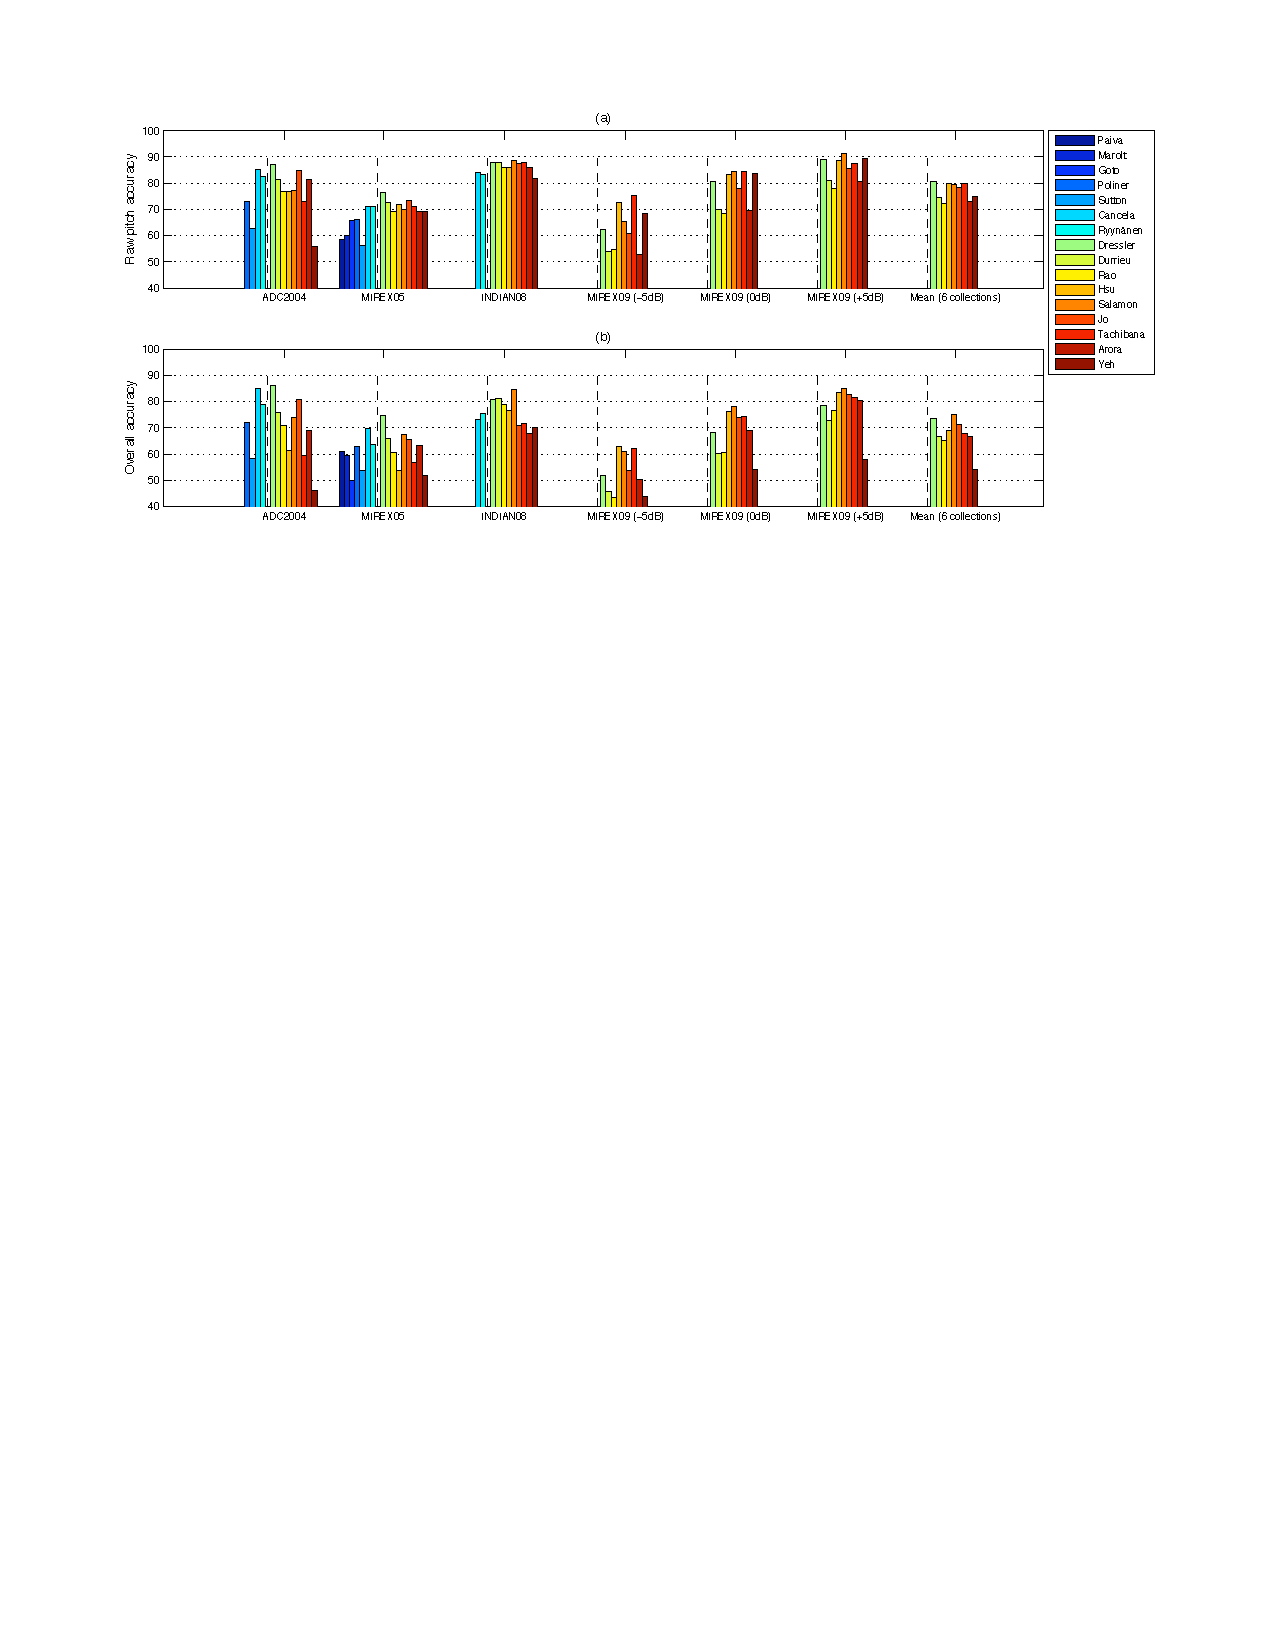
\includegraphics[width=1.1\textwidth]{Figures/comparisonall}
      \caption{a) Raw pitch accuracy and b) overall accuracy obtained in MIREX by 16 melody extraction algorithms evaluated in~\cite{comparison}. The vertical dashed line separates the algorithms that were only evaluated on some collections (left of the line) from those evaluated on all six collections (right of the line)~\cite{comparison}.}
\label{fig:comparison}
\end{figure}


In Figure~\ref{fig:comparison}. the authors presented results obtained by the algorithms evaluated at MIREX. To get a general idea of the performance of the algorithms, it is sufficient to focus on two evaluation measures.
The raw pitch accuracy, presented in Figure~\ref{fig:comparison} a) represents how well the algorithm tracks the pitch of the melody. The overall accuracy on the other hand, as shown in Figure~\ref{fig:comparison} b), combines this measure with the efficiency of the algorithm's voicing detection, meaning the voicing-related measures are also reflected in this measure.

As we can see, some collections are universally hard to analyse (for example MIREX09 -5db). In general the collections yield different results for different algorithms. This allows us to spot pros and cons of each approach investigated.

We can also notice that the raw pitch accuracy gradually improved from 2005 to 2009. Overall we can see that the average pitch accuracy over a collection lies between 70--80\%.

On the other hand, when it comes to overall accuracy, the performance is lower compared to the raw pitch accuracy for all algorithms due to voicing detection being factored into the results. The importance of performance of this step depends on the intended use of the algorithm. Generally, the overall accuracy results lie between 65--70\%.

Finally, an important factor in assessment of an algorithm is its complexity. While deriving O-notation is too complex for some of the algorithms, generally it is observed that algorithms involving source separation are significantly more computationally complex than salience based approaches Unfortunately, there is no specific data provided by Salamon and G\'{o}mez [9] or by Durrieu [5] on their algorithms.

In conclusion, we believe the solution proposed by Salamon and G\'{o}mez could be better fitted to the purpose of this project. It outperforms the algorithm created by Durrieu, as seen in Figure~\ref{fig:comparison}, however, this is based only on the data used by MIREX to evaluate the algorithms, which might not align with our needs. In addition to this, as we are developing a game, accuracy of the algorithm is of crucial importance and even if one algorithm is performing slightly better than the other in terms of accuracy, we would still have to consider the time it would require the user to wait for their playable song to be generated. 

\newpage


\section{Introduction to Neural Networks}
\vspace{10pt}

An Artificial Neural Network (ANN) is an information processing paradigm that can be thought of as humans' attempt to simulate the brain electronically. Its first conceptual model was developed by Warren S. McCulloch, a neuroscientist, and Walter Pitts, a logician, in 1943. In their paper, ``A Logical Calculus of the Ideas Imminent in Nervous Activity'', they describe the concept of a neuron, a single cell living in a network of cells that receives inputs, processes those inputs, and generates an output~\cite{firstNN}. Their work served as foundation for designing a computational model based on the brain to solve certain kinds of problems.

Neural networks, with their remarkable ability to derive meaning from complicated or imprecise data, can be used to extract patterns and detect trends that are too complex to be noticed by either humans or other computer techniques. Their most common application in computing today is to perform ``easy-for-a-human, difficult-for-a-machine'' tasks, often referred to as pattern recognition. Thanks to being implemented on computers, they have higher computational capabilities than any human being - calculating a cube of 9124 in memory is not straightforward for us, but a computer can come up with an answer almost immediately. On the other hand, thanks to their structure, neural networks can tackle problems not easy to solve by a simple computer running sequential code, like facial recognition or regression analysis.

A trained neural network can be thought of as an ``expert'' in the category of information it has been given to analyse. This expert can then be used to provide projections given new situations of interest and answer ``what if'' questions.

\vspace{10pt}

\subsection{Models}

\begin{wrapfigure}{l}{0.5\textwidth}
  \vspace{-30pt}
  \begin{center}
    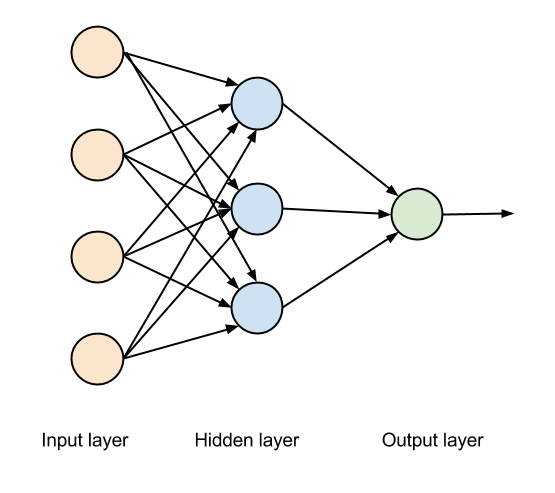
\includegraphics[width=0.48\textwidth]{Figures/simpleANN}
  \end{center}
  \caption{Diagram of a simple neural network with 4 input nodes, 3 nodes in a hidden layer and one output node.}
  \label{fig:examplennn}
\end{wrapfigure}


The computational systems we usually write are procedural -- a program starts at the first line of code, executes it, and goes on to the next, following instructions in a linear fashion.
On the other hand, neural network are ``connectionist'' computational systems. A true neural network does not follow a linear path. Instead, the information is processed collectively, in parallel throughout a network of neurons.

Neural networks are made up of many artificial neurons. There are many different ways of connecting them to create a neural network and the number of neurons depends on a task the network is designed for.

An example system depicted in Figure~\ref{fig:examplennn} has three layers. The first layer has input neurons (marked red) which send data via synapses to the second layer of neurons (colour blue). Each input going into the neuron has its own weight associated with it. A weight is simply a floating point number and modifying it allows us to adjust our network to improve the training outcome. The weights in most neural nets can be both positive and negative, therefore providing excitatory (carrying information) or inhibitory (regulating the activation of excitatory neurons) influences to each input. 

As each input enters the nucleus, it is multiplied by its weight. The nucleus then sums all these new input values which gives us the activation. If the activation is greater than a threshold value, the neuron outputs a signal. If the activation is less than the threshold, the neuron outputs zero. This is typically called a step function.

One type of neural network is called a feedforward network named after the way the neurons in each layer feed their output forward to the next layer until we get the final output from the neural network. 
 
Each input is sent to every neuron in the hidden layer (marked blue) and then each hidden layer’s neuron’s output is connected to every neuron in the next layer. There can be any number of hidden layers within a feedforward network but one is usually enough to suffice for most problems. There can be any number of neurons in each layer, depending on the problem that is being solved.

\vspace{10pt}

\subsection{Training}
Once a network has been structured for a particular application, it is ready to be trained. In the beginning, the initial weights are chosen randomly. 
There are two approaches to training -- supervised and unsupervised. Supervised training involves a mechanism of providing the network with the desired output either by manually ``grading'' the network's performance or by providing the desired outputs with the inputs. Unsupervised training is where the network has to make sense of the inputs without outside help.

Majority of networks utilise supervised training. Unsupervised training is used to perform some initial characterisation on inputs~\cite{mostcommon}.

\vspace{10pt}

\subsection*{Supervised Training}

In supervised training, both the inputs and the outputs are provided. The network then processes the inputs and compares its resulting outputs against the desired outputs. Errors are then propagated back through the system, causing the system to adjust the weights which control the network. This process occurs over and over as the weights are continually tweaked. The set of data which enables the training is called the ``training set''. During the training of a network the same set of data is processed many times as the connection weights are ever refined.

Unfortunately, some networks never learn. This can be caused by the input data not containing the specific information from which the desired output is derived. Networks can also fail to converge if there is not enough data to enable complete learning. 

Ideally, there should be enough data so that part of the data can be held back as a test. Many layered networks with multiple nodes are capable of memorising data. To make sure the network is learning significant patterns rather than plainly memorising the data, supervised training needs to hold back a set of data to be used to test the system after it has undergone its training.

If a network simply cannot solve the problem, the designer then has to review the input and outputs, the number of layers, the number of elements per layer, the connections between the layers, the summation, transfer, and training functions, and even the initial weights themselves. Those changes required to create a successful network constitute a process where the ``art'' of neural networking occurs.

Another part of the designer's creativity governs the rules of training. There are many algorithms used to implement the adaptive feedback required to adjust the weights during training. The most common technique is backward-error propagation, more commonly known as backpropagation, which we will describe later.

Yet, training is not just a technique. It involves a ``feel'', and conscious analysis, to insure that the network is not over-trained. Initially, an artificial neural network configures itself with the general statistical trends of the data. Later, it continues to ``learn'' about other aspects of the data which may be spurious from a general viewpoint.

When finally the system has been correctly trained, and no further learning is needed, the weights can, if desired, be saved. This way it can be used for predicting the output values for new, unseen data.

\vspace{10pt}

\subsection*{Unsupervised Training}

The other type of training is called unsupervised training. In unsupervised training, the network is provided with inputs but not with desired outputs. The system itself must then decide what features it will use to group the input data. This is often referred to as self-organisation or adaption.

At the present time, unsupervised learning is not well understood. This adaption to the environment is the promise which would enable science fiction types of robots to continually learn on their own as they encounter new situations and new environments~\cite{unsupervised}.

Unfortunately, life is filled with situations where we are unable to extract and provide useful and valid training sets. Some of these situations could involve military action where new combat techniques and new weapons might be encountered. This unexpectedness of life and our desire to be prepared for every eventuality, there continues to be research into this field, bringing hope for future discoveries.

\vspace{10pt}

\subsection{Backpropagation Algorithm}

\begin{wrapfigure}{r}{0.5\textwidth}
  \vspace{-30pt}
  \begin{center}
    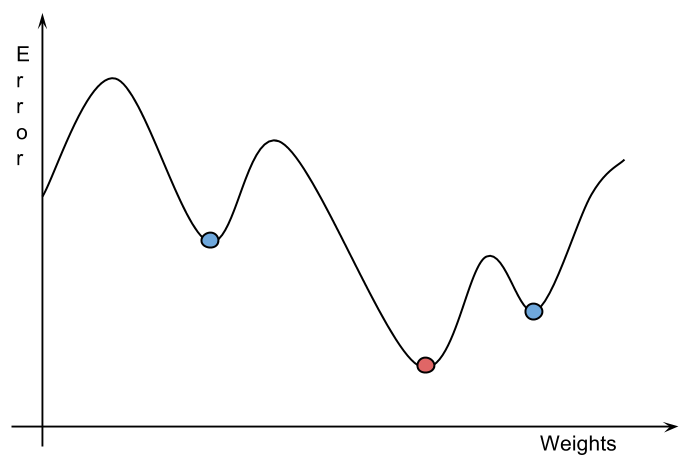
\includegraphics[width=0.48\textwidth]{Figures/localminima}
  \end{center}
  \caption{Diagram depicting the problem of the local minima. The x axis represents the weights and the y axis stands for the value of the error function per epoch. As the algorithm is greedy, once it hits the first minimum it will fail to reach the global minimum (red) due to the increase in the error it would have to experience~first.}
  \label{fig:localminima}
\end{wrapfigure}

A backpropagation network is a network that learns by example. Given the desired input and output data telling the network what we want it to do, it changes its weights so that, when training is finished, it produces the required output for a particular input. Backpropagation networks are ideal for Pattern Recognition and Mapping Tasks.

The algorithm starts by first setting up all the network's weights to be small random numbers. Next, the input pattern (multiplication by the weights) is applied and the output calculated. This stage is called the \textit{forward pass}. The calculation is likely to give an output which is completely different to what we passed in as the expected value, since all the weights are random. The error of each neuron is calculated \textit{(expected output -- actual output)}. This error is then used mathematically to change the weights in such a way that the error will get smaller. In other words, the actual input of each neuron will get closer to its expected output. This  part is called the \textit{reverse pass}. The process is repeated again and again until the error is minimal.

Backpropagation algorithm has some problems associated with it. Perhaps the best known is connected to local minima. This occurs because the algorithm always changes the weights in such a way as to cause the error to fall. But the error might briefly have to rise as part of a more general fall. If this is the case, the algorithm will ``get stuck'' (because it cannot go uphill) and the error will not decrease further. This is depicted in Figure~\ref{fig:localminima}.

There are are several solutions to this problem. One is very simple and that is to reset the weights to different random numbers and try training again (this can also solve several other problems). Another solution is to add ``momentum'' to the weight change. This means that the weight change this iteration depends not just on the current error, but also on previous changes. For example: 
\begin{equation}
W+ = W + Current\; change + (Change\; on \;previous\; iteration * constant)
\end{equation}

\vspace{20pt}


\section{Mood Detection}
\vspace{10pt}

It is well known that music can convey emotion and modulate mood. That is why the relation between musical sounds and their influence on the listener’s emotion has been well studied.

In this section we talk about different means of describing the mood -- from discrete classification to defining a variable with continuous value. In addition to this, we go over relevant existing literature describing different attempts of designing a system capable of extracting emotions from music tracks.

\subsection{Emotion Classification}
\label{sec:emotionClass}

Currently, there is no standard method to measure and analyse emotion in music. However, a psychological model of emotion has found increasing use in computational studies. 

In 1989, in his publication~\cite{Russell}, J. A. Russell noticed that set of emotional dimensions such as displeasure, distress, depression, excitement etc. are interrelated in a highly systematic fashion. He claimed these relationships can be represented in a spacial model in which concepts fall in circle in the following order: pleasure, excitement, arousal, distress, displeasure, depression, sleepiness and relaxation. Depiction of the model is presented in Figure~\ref{fig:Russell}.

\begin{figure}[b]
        \centering
        \begin{subfigure}[b]{0.47\textwidth}
                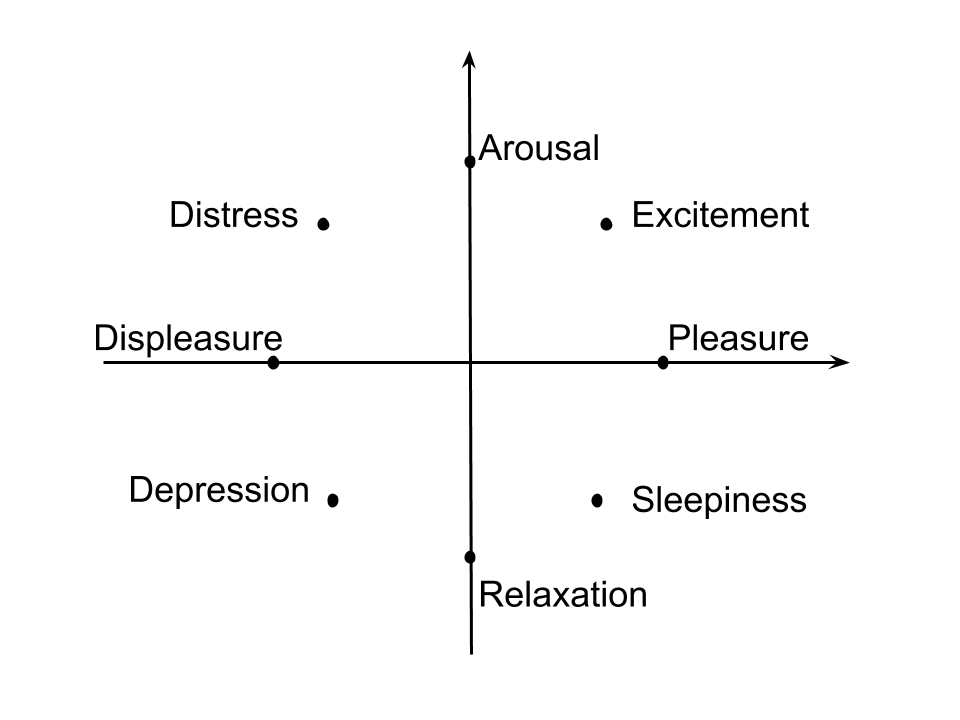
\includegraphics[width=\textwidth]{Figures/Russell}
                \caption{Model proposed by J. A. Russell.}
                \label{fig:Russell}
        \end{subfigure}%
        ~ %add desired spacing between images, e. g. ~, \quad, \qquad, \hfill etc.
          %(or a blank line to force the subfigure onto a new line)
        \begin{subfigure}[b]{0.47\textwidth}
                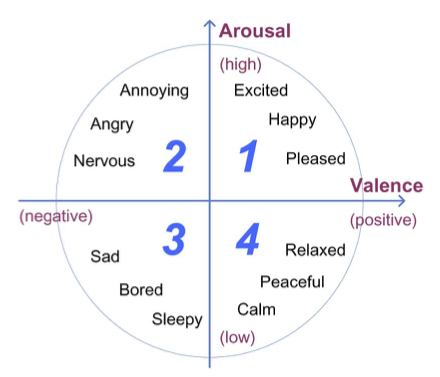
\includegraphics[width=\textwidth]{Figures/ThayersAV}
                \caption{Model proposed by R. E. Thayer~\cite{mood}.}
                \label{fig:Thayer}
        \end{subfigure}
          \caption{Diagram of both models for representing emotions.}
        ~ %add desired spacing between images, e. g. ~, \quad, \qquad, \hfill etc.
        \label{fig:RussellThayer}
\end{figure}


A somewhat similar model was described in 1989 by R. E. Thayer. Thayer’s two-dimensional emotion model offers a simple but quite effective model for placing emotion in a two-dimensional space~\cite{Thayer}. In the model, the amount of arousal and valence is measured along the vertical and horizontal axis, respectively.

Diagram~\ref{fig:Thayer} depicts the relation between valence and arousal values and the moods perceived by people. As we can see, the high arousal is connected to how energetic the music is, whereas valence refers to how positive (or negative) the emotions in the track are. 

\vspace{10pt}

\subsection{Related Literature}

Thanks to music's ability to affect people's emotions, much research went into discovering which feature was responsible for this. As there is no measure of ``mood'' alone, scientists tried different approaches in defining the emotions and their cause.

Some studies have explored the relationship between physiological activity experienced by a listener and perceived emotion, be it facial expression or speech recognition of even heartbeat and respiratory changes~\cite{physicalmood}.
Others have explored the relationship between perceived emotion and the musical/acoustic features themselves.

One of the first publications on emotion detection in music is credited to Feng, Zhuang, and Pan~\cite{moodold}. They employed Computational Media Aesthetics, that is, analysis of two music dimensions to detect mood for music information retrieval tasks. The two dimensions -- tempo and articulation, were extracted from the audio signal and mapped to one of four emotional categories; happiness, sadness, anger, and fear. 
After that, they calculated a feature called relative tempo. Once the mean and standard deviation of the feature called average silence ratio in the computational articulation model was calculated, a simple backpropagation neural network classifier was trained to detect mood.

Different approach was applied by Kim and Andr\'{e}~\cite{physicalmood}. To collect physiological data set, they used musical induction which led people participating in the research to real emotional states. This collection process was run over many weeks to exclude external emotional impact. Then the researches used four-channel biosensors to measure electromyogram, electrocardiogram, skin conductivity, and respiration changes. From that, they retrieved and analysed a wide range of physiological features to find the best emotion-relevant ones and correlated them with emotional states. Finally, the researchers performed the classification of four musical emotions (positive/high arousal, negative/high arousal, negative/low arousal, and positive/low arousal) by using an extended linear discriminant analysis (pLDA).

In publication by Yang, Lin, Su and Chen~\cite{mood}, the authors presented a tool which recognises a mood in a musical track, allowing a user to then choose the song they want to play by deciding on emotions it is supposed to represent. Specifically, the authors formulated music emotion recognition as a regression problem to predict the arousal and valence values (AV values) of each music sample directly. For this purpose, they adopted Support Vector Regression (SVR) as a classifier using a number of chosen features.

Potentially, the treating mood recognition as a regression problem seems more appropriate for our project as it allows for better granularity in the melody emotion detection and, hence, wider variety of changes in the game's environment.

\vspace{20pt}

\section{Song Structure Retrieval}
\vspace{10pt}

Automatic music structure analysis from audio signals is an interesting topic that receives a lot of attention these days. The technique can be used for music data analysis, indexing, retrieval and management. It decomposes a song into several sections and detects repetitive patterns.

\begin{figure}[h]
	\centering
   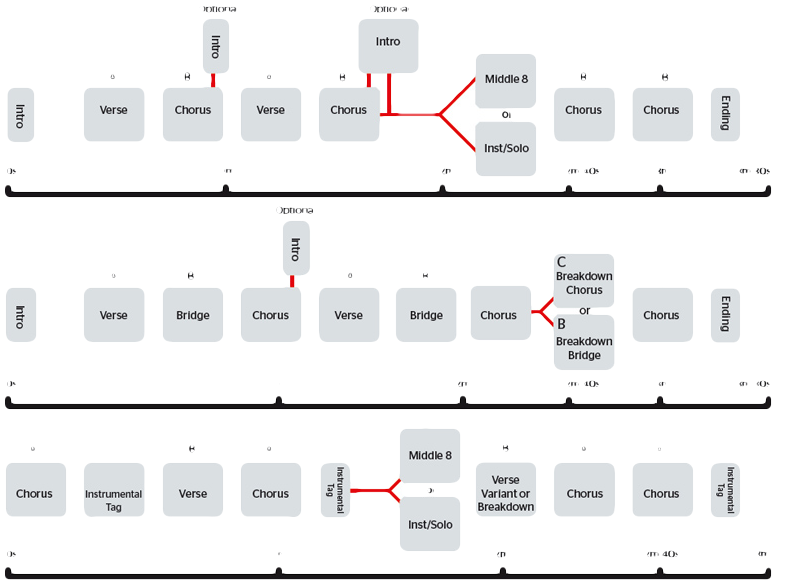
\includegraphics[width=0.9\textwidth]{Figures/songstructure}
  \caption{An example diagram of two different song structures.}
\end{figure}


\vspace{10pt}

\subsection{Song Structure}



Popular music is typically created using sectional, repeating forms. 
Most pop/rock songs have a standard structure: an introduction followed by alternating verses, choruses, and solos/bridges segments, and concluding with an outro. A musical boundary can be defined as the point in time where a song transitions between two of these segments.

However, this is not always the case as there are different types of musical structure. To describe them, let us represent the verse as A and the chorus as B. 

Songs could be \textit{strophic} -- where all the verses are written to the same music, which could be represented as AAA... . Many folk and popular songs represent a strophic structure, including ``Barbara Allen'', ``Erie Canal'', and ``Michael Row the Boat Ashore''~\cite{strophic}.

Another song structure seen in the pop culture is \textit{thirty-two-bar} form, where the structure of each repeated part is made up of four eight bar sections, in an AABA pattern. An example of a song with such a structure could be The Rolling Stones' ``Brown Sugar'' or The Police's ``Every Breath You Take''~\cite{32bar}. 

In contrast to thirty-two-bar form, which is focused on the verse (contrasted and prepared by the B section), in \textit{verse–chorus} form it is the chorus that is highlighted (prepared and contrasted with the verse). Good example could be a song ``Be My Baby'' first recorded by The Ronettes, where the structure could be represented by ABABB(B)~\cite{32bar}.



\subsection{Similarity Matrix}

A similarity matrix is a matrix of scores that represent the similarity between a number of data points. Each element of the similarity matrix contains a measure of similarity between two of the data points. Similarity matrices are strongly related to their counterparts, distance matrices and substitution matrices.
Similarity matrices have a wide range of uses, including finding clusters of data points.

Similarity between two points $i, j$ is computed as a distance between the features of the beat indices $i$ and $j$. There are many ways of computing a distance. Some of the most popular are:
\begin{description}
\item[Euclidean] --  for two vectors of attributes, $p$ and $q$, in an $n$-dimensional real vector space, the Euclidean distance between them is calculated as:
\begin{equation}
d(p, q) = \sqrt{(p_1- q_1)^2 + (p_2 - q_2)^2+\cdots+(p_i - q_i)^2+\cdots+(p_n - q_n)^2}
\end{equation}
\item[Cosine] --  for two vectors of attributes, $p$ and $q$, in an $n$-dimensional real vector space, the cosine distance is represented using a dot product and magnitude as:
\begin{equation}
d(p, q) = {p \cdot q \over \|p\| \|q\|} = \frac{ \sum\limits_{i=1}^{n}{p_i \times q_i} }{ \sqrt{\sum\limits_{i=1}^{n}{([_i)^2}} \times \sqrt{\sum\limits_{i=1}^{n}{(q_i)^2}} }
\end{equation}
\item[Manhattan] --  for two vectors of attributes, $p$ and $q$, in an $n$-dimensional real vector space with fixed Cartesian coordinate system, the Manhattan distance is represented as the sum of the lengths of the projections of the line segment between the points onto the coordinate axes:
\begin{equation}
d(p, q) = \|p - q\|_1 = \sum_{i=1}^n |p_i-q_i|,
\end{equation}
\item[Correlation] --  for two vectors of attributes, $p$ and $q$, in an $n$-dimensional real vector space, the correlation distance is defined as:
\begin{equation}
d(p, q) =  {(p - \mu _{p}) \cdot (q - \mu _{q}) \over ||p -\mu _{p} ||_{2} ||q - \mu _{q}||_{2}}
\end{equation}
where $|| \cdot ||_{2}$ stands for the Euclidean distance, $\mu _{x}$ denotes the mean of the feature vector x, and $\cdot$ represents the dot product.
\end{description}

\vspace{10pt}


\vspace{10pt}

\subsection{Related Literature}

Many other researchers have considered the importance of patterns and repetition in music. This led to development of many algorithms for the task.


For instance, Foote~\cite{Foote} proposed the use of a self-similarity matrix (SSM for short) to visualise similarities between segments of music signals. In their algorithm, given a song, each element of a SSM represents the pairwise similarity between two respective temporal windows of acoustic features. Furthermore, Foote and Cooper~\cite{FooteCooper} developed a music segmentation technique using an audio novelty measure. That is, the local similarity of adjacent musical signals within a coherent section is used to determine section boundaries. Then, all detected sections are compared with each other for their pairwise similarity and clustered into different patterns. To achieve that, a Gaussian-tapered ``checkerboard'' kernel is correlated along the main diagonal of the SSM.  Peaks in the correlation indicate locally novel audio.


\begin{wrapfigure}{rb}{0.5\textwidth}
  \begin{center}
    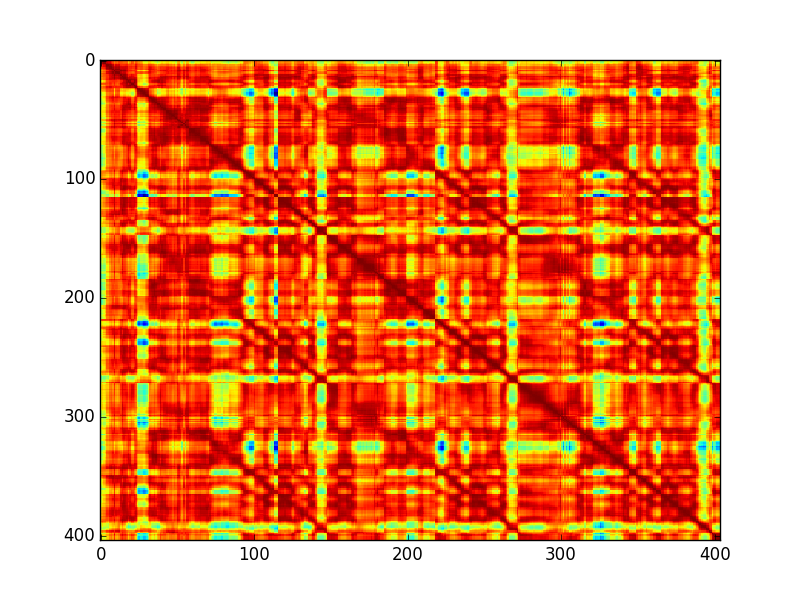
\includegraphics[width=0.48\textwidth]{Figures/mfcc_no_log_sync}
  \end{center}
  \caption{Self similarity matrix computed using MFCC feature for ``Help'' by The Beatles.}
  \label{fig:SSMbach}
\end{wrapfigure}

Many researchers developed their methods on top of this solution, approaching the problem of the segments grouping from different angles. Some were using Gaussian Mixture Models (GMM) -- a probabilistic model that assumes all the data points are generated from a mixture of a finite number of Gaussian distributions with unknown parameters. 

Another approach seen in literature is a variant of the Nearest Neighbour Search (NSS), also known as similarity search or closest point search. NSS is an optimisation problem for finding the closest (or most similar) points. Closeness is typically expressed in terms of a dissimilarity function: the less similar the objects, the larger the function values. Formally, the NSS problem is defined as follows: given a set $S$ of points in a space $M$ and a query point $q \in M$, find the closest point in $S$ to $q$.

Finally, a Non-negative Matrix Factorisation (NMF) can be applied to group the segments, as presented by Kaiser and Sikora~\cite{Sikora}. Non-negative matrix approximation is a group of algorithms in multivariate analysis and linear algebra where a matrix $V$ is factorised into (usually) two matrices $W$ and $H$, with the property that all three matrices have no negative elements. This non-negativity makes the resulting matrices easier to inspect. Also, in applications such as processing of audio spectrograms non-negativity is inherent to the data being considered. As the problem is not exactly solvable in general as the problem has been shown to generalize the k-means clustering problem (which is known to be NP-complete). That is why it is commonly approximated numerically~\cite{NMFNP}.

Nieto and Jehan~\cite{Nieto} based their approach on the NMF method, extending it by adding a convex constrain that results in weighted cluster centroids, representing the different sections of a musical piece in a more effective manner. 
In standard NMF, matrix factor $W \in \Re^{m \times k}_{+}$, i.e., $W$ can be anything in that space. Convex NMF restricts $W$ to a be convex combination of the input data vectors  $(v_1, \cdots, v_n)$. This greatly improves the quality of data representation of $W$. Furthermore, the resulting matrix factor $H$ becomes more sparse and orthogonal. Once they obtained the decomposition matrices, Nieto and Jehan efficiently extracted music boundaries by clustering the decomposition matrices, which take into account the repeated parts across the song instead of just detecting sudden local changes.

Some researchers joined their methods for grouping and boundary identification into one algorithm. For instance, Levy and Sandler used Hidden Markov Models (HMM), a generative probabilistic model, in which a sequence of observable $X$ variables is generated by a sequence of internal hidden state $Z$. The hidden states cannot be observed directly and the transitions between hidden states are assumed to have the form of a (first-order) Markov chain. They can be specified by the start probability vector $\Pi$ and a transition probability matrix $A$. The emission probability of an observable can be any distribution with parameters $\Theta_{i}$ conditioned on the current hidden state (e.g. multinomial, Gaussian). The HMM is completely determined by $\Pi$, $A$ and $\Theta_{i}$.

Another approach was presented by Peeters, La Burthe, and Rodet. In their paper~\cite{Peeters}, they presented an algorithm which makes use of k-means clustering. The k-means clustering is a method of vector quantisation, originally from signal processing. It aims to partition n observations into $k$ clusters in which each observation belongs to the cluster with the nearest mean, serving as a prototype of the cluster. This results in a partitioning of the data space into Voronoi cells (a partitioning of a plane into regions based on distance to points in a specific subset of the plane).
As we mentioned earlier, the problem is computationally difficult (NP-hard). However, there are efficient heuristic algorithms that are commonly employed and converge quickly to a local optimum.

An alternative to using any variants of SSM is using supervised learning. For instance, Turnbull and Lanckriet~\cite{segmentsupervised} developed a set of difference features that indicate when there are changes in perceptual aspects (e.g., timbre, harmony, melody, rhythm) of the music. They used multiple individual difference features to detect boundaries of a song. 

\vspace{20pt}

\section{Gameplay Generation}

It is not really surprising that there is no current literature on the problem of automatically mapping melody to a series of buttons given an arbitrary piece of music. Most of the games available on the market are released with predetermined sets of songs, with sequences of buttons manually designed by the creators. This approach enables the developers to ensure high quality of the gameplay but limits the potential experience and discourages people whose music taste differs from fans of the most popular and generic music. 

Any other releases or fan-made patches that enable the users to play to a wider range of music, focus on rhythmic representation of the song, disregarding the fundamental frequency of the main melody.

However, we believe an algorithm can be developed where the buttons can be mapped to the $f_{0}$ in the main melody extracted by main melody extraction algorithm. Such algorithm should produce a consistent output that makes the gameplay as intuitive for the user as possible.